% 第 1 章 向量空间 (Vektorräume)
\chapter{向量空间}\index{xiangliangkongjian@向量空间(Vektorraum; K-Vektorraum)}

\section*{预备说明}

\emph{平面}(\textup{Ebene})\index{pingmian@平面(Ebene)}内或三维空间中的具体几何问题, 常常是许多重要数学发展的出发点.作为处理这类问题的工具, 人们发展出了诸如借助圆规\emph{和}(\textup{Summe})\index{he@和(Summe)}直尺的几何作图方法.另一种策略则是把几何问题转化为计算问题, 以便通过"计算"来获得解答.这正是\emph{解析几何}(\textup{analytische Geometrie})\index{jiexijihe@解析几何(analytische Geometrie)}的做法, 它于 1637 年由勒内·\emph{笛卡尔}(\textup{Descartes, R.})\index{dikaer@笛卡尔(Descartes, R.)}(René Descartes)在其著名的著作"几何学"(La G\'eom\'etrie)中奠定.而解析几何的许多计算方法, 今天又以扩展的形式被概括在线性\emph{代数}(\textup{Algebra; R-Algebra})\index{daishu@代数(Algebra; R-Algebra)}的概念之下.

下面我们想较为仔细地谈谈笛卡尔方法的\emph{基}(\textup{Basis})\index{ji@基(Basis)}本思想.为此, 我们考虑一个平面 $E$(比如在我们周围的三维空间中的平面), 把 $E$ 中的一点 $0$ 标为所谓的原点, 然后选取一个\emph{坐标}(\textup{Koordinaten})\index{zuobiao@坐标(Koordinaten)}系, 其坐标轴 $x$ 和 $y$ 在原点 $0$ 处相交.若再把坐标轴 $x$ 和 $y$ 分别与实数集 $\mathbb{R}$ 等同起来, 那么 $E$ 的点 $P$ 就可以解释为实数对:

\begin{center}
\begin{tikzpicture}[>=latex, scale=1.15]
  \draw[->] (-0.3,0) -- (4.4,0) node[right]{$x$};
  \draw[->] (0,-0.3) -- (0,3.4) node[above]{$y$};
  \fill (0,0) circle (1.6pt) node[below left]{$0$};
  \coordinate (P) at (3.1,2.2);
  \fill (P) circle (1.6pt) node[above right]{$P = (x_1, y_1)$};
  \draw[dashed] (P) -- (3.1,0) node[below]{$x_1$};
  \draw[dashed] (P) -- (0,2.2) node[left]{$y_1$};
\end{tikzpicture}
\end{center}

事实上, 若 $P$ 是 $E$ 中的一点, 那么过 $P$ 作 $y$ 轴的平行线, 它与 $x$ 轴交于一点 $x_1$; 相应地, 过 $P$ 作 $x$ 轴的平行线与 $y$ 轴交于一点 $y_1$, 于是从 $P$ 得到坐标对 $(x_1, y_1)$.反过来, 也可以从坐标对 $(x_1, y_1)$ 简单地还原出 $P$, 它就是过 $x_1$ 的 $y$ 轴平行线与过 $y_1$ 的 $x$ 轴平行线的交点.更准确地说, 我们注意到, 对应 $P \longmapsto (x_1, y_1)$ 在 $E$ 的点与实数对之间建立了可逆的一一对应\emph{关系}(\textup{Relation})\index{guanxi@关系(Relation)}, 因此正如所说, 我们可以进行如下等同:

\[
E = \mathbb{R}^2 = \{\text{一切实数对}\}.
\]

当然, 这种等同依赖于原点 $0$ 以及坐标轴 $x, y$ 的选取.在上图中我们画出了一个直角坐标系.不过原则上, 在现阶段我们还完全不需要知道有关角度的任何知识.只需取两条经过原点 $0$ 的不同\emph{直线}(\textup{Gerade})\index{zhixian@直线(Gerade)} $x$ 和 $y$ 作为坐标轴就够了.对此的进一步说明将在第 2 章的预备说明中给出.

这里还要把两条坐标轴 $x, y$ 与实数集 $\mathbb{R}$ 的等同说得更仔细一些.固定原点之后, 在 $x$ 和 $y$ 上各自定义了以 $0$ 为中心,以某个实数作为伸缩因子的伸缩\emph{映射}(\textup{Abbildung})\index{yingshe@映射(Abbildung)}.例如在 $x$ 上取一个非零的点 $1_x \in x$, 并用 $\alpha \cdot 1_x$ 表示 $1_x$ 在伸缩因子为 $\alpha$ 的伸缩下的\emph{像}(\textup{Bild})\index{xiang@像(Bild)}, 那么 $x$ 恰好由所有点 $\alpha \cdot 1_x$ 组成, 其中 $\alpha$ 遍历全体实数.更确切地说, 对应 $\alpha \longmapsto \alpha \cdot 1_x$ 在实数与 $x$ 的点之间建立了一一对应.类似地, 在 $y$ 上取非\emph{零点}(\textup{Nullstelle})\index{lingdian@零点(Nullstelle)} $1_y \in y$ 之后, $x$ 与 $y$ 就自然地与实数集 $\mathbb{R}$ 等同起来, 其中 $0, 1_x \in x$ 与 $0, 1_y \in y$ 分别对应于实数 $0$ 和 $1$.然而, 点 $1_x \in x$ 与 $1_y \in y$ 的自由选取, 以及使用不一定是直角坐标系的可能性, 都提醒我们一个困难: 在等同 $E = \mathbb{R}^2$ 之下, $E$ 中两点间的距离未必等于 $\mathbb{R}^2$ 上通常的欧几里得距离, 后者对两点 $P_1 = (x_1, y_1)$ 与 $P_2 = (x_2, y_2)$ 由

\[
d(P_1, P_2) = \sqrt{(x_1 - x_2)^2 + (y_1 - y_2)^2}
\]

给出.要在 $E$ 上正确地反映距离, 需要借助我们后面还要讨论的\emph{数量积}(\textup{Skalarprodukt})\index{shuliangji@数量积(Skalarprodukt)}.

在数学中, 人们总是力求在分析自己感兴趣的现象与问题时, 归结到某些"简单的基本结构", 这些结构正是所观察现象的根源.这样被认识为重要的基本结构, 往往脱离实际问题本身来研究, 以便弄清楚它们会带来什么影响; 人们把这称为研究一个\emph{模型}(\textup{Modell})\index{moxing@模型(Modell)}.\emph{模}(\textup{Modul})\index{mo@模(Modul)}型的优点是通常更容易看清楚, 但有时也有缺点: 它可能只能从某些侧面来描述真正要研究的情形.

在我们的情形中, 笛卡尔方法带来的认识是: 直线,平面或三维空间中的点可以用坐标来描述.在此基础上, 正如我们所看到的, 可以把一切实数对构成的\emph{集合}(\textup{Menge})\index{jihe@集合(Menge)} $\mathbb{R}^2$ 看作一个平面的模型.相应地, 一切实数三\emph{元组}(\textup{n-Tupel})\index{yuanzu@元组(n-Tupel)}构成的集合 $\mathbb{R}^3$ 构成三维空间的模型, 而 $\mathbb{R} = \mathbb{R}^1$ 自然构成一条直线的模型.对这些模型的研究把我们引向本章的中心主题, 即\emph{向量空间}(\textup{Vektorraum; K-Vektorraum})\index{xiangliangkongjian@向量空间(Vektorraum; K-Vektorraum)}.\emph{向量}(\textup{Vektor})\index{xiangliang@向量(Vektor)}空间作为基本结构含有两种运算: 一是纯量与(在我们情形下为实数)向量的乘法, 它可以设想为一个伸缩过程; 二是向量的加法.我们想以平面 $E$ 及其模型 $\mathbb{R}^2$ 为例, 来说明这一点及其相应的几何结论.

我们从数乘开始.对

\[
\alpha \in \mathbb{R}, \qquad P = (x_1, y_1) \in \mathbb{R}^2
\]

把

\[
\alpha \cdot P = \alpha \cdot (x_1, y_1) := (\alpha x_1, \alpha y_1)
\]

称为 $\alpha$ 与 $P$ 的乘积, 在 $E$ 中它给出如下的图形:

\begin{center}
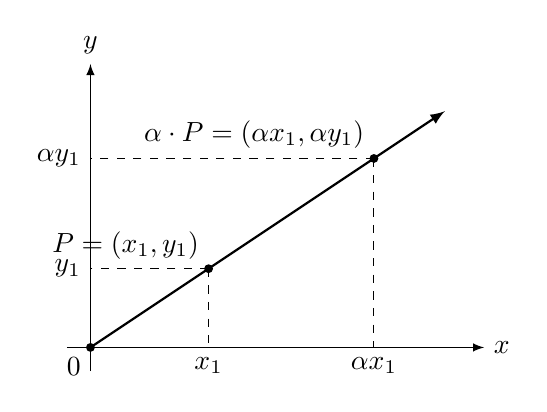
\begin{tikzpicture}[>=latex]
  \draw[->] (-0.3,0) -- (5.0,0) node[right]{$x$};
  \draw[->] (0,-0.3) -- (0,3.6) node[above]{$y$};
  \fill (0,0) circle (1.6pt) node[below left]{$0$};
  \coordinate (P) at (1.5,1.0);
  \coordinate (aP) at (3.6,2.4);
  \draw[dashed] (P) -- (1.5,0) node[below]{$x_1$};
  \draw[dashed] (P) -- (0,1.0) node[left]{$y_1$};
  \draw[dashed] (aP) -- (3.6,0) node[below]{$\alpha x_1$};
  \draw[dashed] (aP) -- (0,2.4) node[left]{$\alpha y_1$};
  \draw[thick, ->] (0,0) -- (4.5,3.0);
  \fill (P) circle (1.6pt) node[above left]{$P = (x_1, y_1)$};
  \fill (aP) circle (1.6pt) node[above left]{$\alpha \cdot P = (\alpha x_1, \alpha y_1)$};
\end{tikzpicture}
\end{center}

因此, 点 $P \in E$ 与纯量 $\alpha \in \mathbb{R}$ 的乘法可以解释为以伸缩中心 $0$,伸缩因子 $\alpha$ 的伸缩映射.若把点 $P \in E$ 看作有向线段意义上的"向量" $\overrightarrow{0P}$, 则这一描述尤其富有启发性.于是向量由它的长度和方向刻画(\emph{零向量}(\textup{Nullvektor})\index{lingxiangliang@零向量(Nullvektor)} $\overrightarrow{00}$ 除外, 它没有确定的方向).向量 $\alpha \cdot \overrightarrow{0P}$ 是由 $\overrightarrow{0P}$ 以因子 $\alpha$ 伸缩而得到的, 即把它的长度乘上 $\alpha$(或者更准确地说, 乘上\emph{绝对值}(\textup{Absolutbetrag})\index{jueduizhi@绝对值(Absolutbetrag)} $|\alpha|$), 其余则保持或反转向量的方向, 视 $\alpha \geq 0$ 还是 $\alpha < 0$ 而定:

\begin{center}
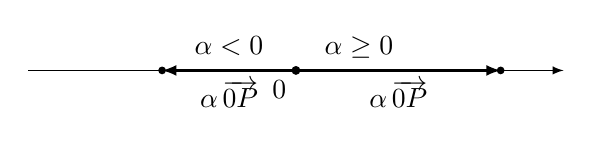
\begin{tikzpicture}[>=latex]
  \draw[->] (-3.4,0) -- (3.4,0);
  \fill (0,0) circle (1.6pt) node[below left]{$0$};
  \draw[thick, ->] (0,0) -- (2.6,0) node[midway,below]{$\alpha\,\overrightarrow{0P}$};
  \fill (2.6,0) circle (1.4pt);
  \draw[thick, ->] (0,0) -- (-1.7,0) node[midway,below]{$\alpha\,\overrightarrow{0P}$};
  \fill (-1.7,0) circle (1.4pt);
  \node[below] at (0.8,0.55) {$\alpha \geq 0$};
  \node[below] at (-0.85,0.55) {$\alpha < 0$};
\end{tikzpicture}
\end{center}

作为另一种运算, 我们考虑 $\mathbb{R}^2$ 中点的加法.对

\[
P_1 = (x_1, y_1), \quad P_2 = (x_2, y_2) \in \mathbb{R}^2
\]

规定

\[
P_1 + P_2 := (x_1 + x_2, y_1 + y_2),
\]

这可在 $E$ 中用如下的草图来说明:

\begin{center}
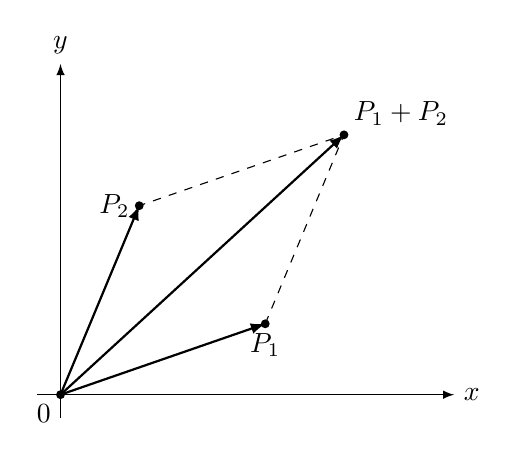
\begin{tikzpicture}[>=latex]
  \draw[->] (-0.3,0) -- (5,0) node[right]{$x$};
  \draw[->] (0,-0.3) -- (0,4.2) node[above]{$y$};
  \fill (0,0) circle (1.6pt) node[below left]{$0$};
  \coordinate (P1) at (2.6,0.9);
  \coordinate (P2) at (1.0,2.4);
  \coordinate (P) at (3.6,3.3);
  \fill (P1) circle (1.6pt) node[below]{$P_1$};
  \fill (P2) circle (1.6pt) node[left]{$P_2$};
  \fill (P) circle (1.6pt) node[above right]{$P_1 + P_2$};
  \draw[thick, ->] (0,0) -- (P1);
  \draw[thick, ->] (0,0) -- (P2);
  \draw[thick, ->] (0,0) -- (P);
  \draw[dashed] (P1) -- (P) -- (P2);
\end{tikzpicture}
\end{center}

同样, 若把向量理解为有向线段, 则 $E$ 中加法的描述也会更富有启发性.不过这里应当允许, 向量作为有向线段可以与自身平行地平移, 从而脱离坐标原点这一天然起点.向量 $\overrightarrow{0P_1}$ 与 $\overrightarrow{0P_2}$ 的和则得到向量 $\overrightarrow{0P}$, 其中 $P$ 是这样得到的终点: 把两个\emph{向量组}(\textup{System von Vektoren})\index{xiangliangzu@向量组(System von Vektoren)}合起来, 即在 $0$ 处接上向量 $\overrightarrow{0P_1}$, 再在 $\overrightarrow{0P_1}$ 的终点 $P_1$ 处接上向量 $\overrightarrow{0P_2}$, 大致如下:

\begin{center}
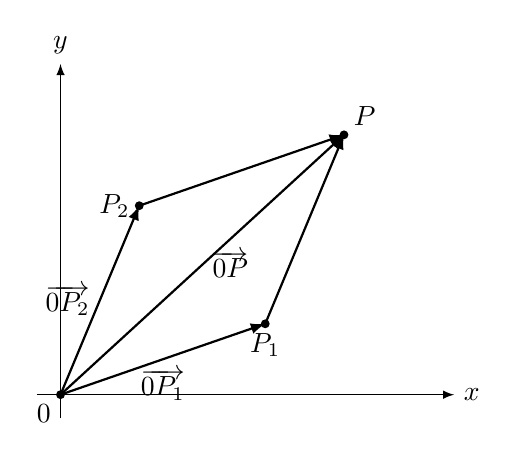
\begin{tikzpicture}[>=latex]
  \draw[->] (-0.3,0) -- (5,0) node[right]{$x$};
  \draw[->] (0,-0.3) -- (0,4.2) node[above]{$y$};
  \fill (0,0) circle (1.6pt) node[below left]{$0$};
  \coordinate (P1) at (2.6,0.9);
  \coordinate (P2) at (1.0,2.4);
  \coordinate (P) at (3.6,3.3);
  \fill (P1) circle (1.6pt) node[below]{$P_1$};
  \fill (P2) circle (1.6pt) node[left]{$P_2$};
  \fill (P) circle (1.6pt) node[above right]{$P$};
  \draw[thick, ->] (0,0) -- (P1) node[midway,below]{$\overrightarrow{0P_1}$};
  \draw[thick, ->] (0,0) -- (P2) node[midway,left]{$\overrightarrow{0P_2}$};
  \draw[thick, ->] (0,0) -- (P) node[midway,right]{$\overrightarrow{0P}$};
  \draw[thick, ->] (P1) -- (P);
  \draw[thick, ->] (P2) -- (P);
\end{tikzpicture}
\end{center}

上述平行四边形构造表明, 如果把向量 $\overrightarrow{0P_2}$ 接在 $0$ 处, 再把向量 $\overrightarrow{0P_1}$ 接在 $\overrightarrow{0P_2}$ 的终点, 加法结果不变.因此向量的加法不依赖于加数的次序, 它是交换的.

我们把 $\mathbb{R}^2$ 的\emph{元素}(\textup{Element})\index{yuansu@元素(Element)}一方面解释为点, 另一方面也解释为有向线段意义上的(可平移的)向量, 这也许会使人有些困惑.原则上, 可以把点与向量的概念加以区分, 办法是把赋给点 $\mathcal{P} \in \mathbb{R}^2$ 的向量 $\overrightarrow{0P}$ 解释为平移 $Q \longmapsto P + Q$, 即 $\mathbb{R}^2$ 到自身的,把元素 $Q \in \mathbb{R}^2$ 映射为 $P + Q$ 的映射.不过我们不打算利用这种可能性, 因为对我们来说, 区分这些概念不会带来好处, 只会把事情复杂化.

接下来我们要说明, $\mathbb{R}^2$ 或 $E$ 中点和向量的加法还会自然地诱导出减法.对 $P_0 = (x_0, y_0) \in \mathbb{R}^2$, 规定

\[
-P_0 = -(x_0, y_0) := (-1) \cdot (x_0, y_0) = (-x_0, -y_0),
\]

并称之为 $P_0$ 的负元素或\emph{逆元}(\textup{inverses Element})\index{niyuan@逆元(inverses Element)}素.它被唯一地表征为满足方程 $P_0 + Q = 0$ 的元素 $Q \in \mathbb{R}^2$.两个元素 $P_1 = (x_1, y_1)$ 与 $P_0 = (x_0, y_0)$ 在 $\mathbb{R}^2$ 中的减法于是很自然地归结为加法:

\[
P_1 - P_0 := P_1 + (-P_0) = (x_1 - x_0, y_1 - y_0).
\]

若再次采用 $E$ 中的向量观点, 那么 $-\overrightarrow{0P_0}$ 由向量 $\overrightarrow{0P_0}$ 反转方向而得到, 其长度保持不变.于是两个向量 $\overrightarrow{0P_1}$ 与 $\overrightarrow{0P_0}$ 的差可以如下表示:

\begin{center}
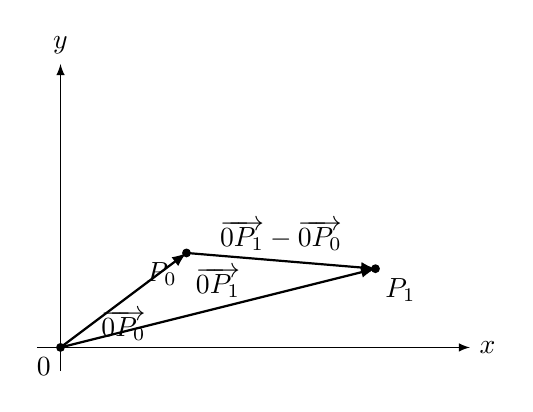
\begin{tikzpicture}[>=latex]
  \draw[->] (-0.3,0) -- (5.2,0) node[right]{$x$};
  \draw[->] (0,-0.3) -- (0,3.6) node[above]{$y$};
  \fill (0,0) circle (1.6pt) node[below left]{$0$};
  \coordinate (P0) at (1.6,1.2);
  \coordinate (P1) at (4.0,1.0);
  \fill (P0) circle (1.6pt) node[below left]{$P_0$};
  \fill (P1) circle (1.6pt) node[below right]{$P_1$};
  \draw[thick, ->] (0,0) -- (P1) node[midway,above]{$\overrightarrow{0P_1}$};
  \draw[thick, ->] (0,0) -- (P0) node[midway,below]{$\overrightarrow{0P_0}$};
  \draw[thick, ->] (P0) -- (P1) node[midway,above]{$\overrightarrow{0P_1} - \overrightarrow{0P_0}$};
\end{tikzpicture}
\end{center}

特别可以看出, 向量 $\overrightarrow{0P_0}$ 与 $\overrightarrow{0P_1} - \overrightarrow{0P_0}$ 的和恰好等于向量 $\overrightarrow{0P_1}$, 这正是合理定义的加法与减法理应做到的.更一般地, 可以作具有如下形式的和

\[
\overrightarrow{0P} = \overrightarrow{0P_0} + \alpha \cdot (\overrightarrow{0P_1} - \overrightarrow{0P_0})
\]

其中 $\alpha \in \mathbb{R}$ 取不同的值.当 $P_0 \neq P_1$ 时, 点 $P$ 总位于由 $P_0$ 和 $P_1$ 确定的直线 $G$ 上, 并且当 $\alpha$ 遍历 $\mathbb{R}$ 时 $P$ 恰好跑遍 $G$:

\begin{center}
\begin{tikzpicture}[>=latex]
  \draw[->] (-0.5,0) -- (5.4,0) node[right]{$x$};
  \draw[->] (0,-0.4) -- (0,3.8) node[above]{$y$};
  \fill (0,0) circle (1.6pt) node[below left]{$0$};
  \coordinate (P0) at (1.4,1.6);
  \coordinate (P1) at (3.8,1.2);
  \coordinate (P) at (2.6,1.4);
  \fill (P0) circle (1.6pt) node[below left]{$P_0$};
  \fill (P1) circle (1.6pt) node[below right]{$P_1$};
  \fill (P) circle (1.6pt) node[above]{$P$};
  \draw[thick] (0.8,1.7) -- (4.4,1.1);
  \node[right] at (4.4,1.1) {$G$};
\end{tikzpicture}
\end{center}

于是, $E$ 或 $\mathbb{R}^2$ 中过给定点 $P_0$ 与 $P_1$ 的直线由方程

\[
G = \{P_0 + t \cdot (P_1 - P_0);\; t \in \mathbb{R}\}
\]

描述.若给定两条这样的直线

\[
G = \{P_0 + t \cdot (P_1 - P_0);\; t \in \mathbb{R}\}, \qquad
G' = \{P_0' + t \cdot (P_1' - P_0');\; t \in \mathbb{R}\}
\]

其中 $P_0 \neq P_1$, $P_0' \neq P_1'$, 那么它们平行当且仅当 $P_1 - P_0$ 是 $P_1' - P_0'$ 的纯量倍(或反之, $P_1' - P_0'$ 是 $P_1 - P_0$ 的纯量倍).若不平行, 则 $G$ 与 $G'$ 恰有一个交点, 而这个交点的计算归结为所谓\emph{线性方程组}(\textup{lineares Gleichungssystem})\index{xianxingfangchengzu@线性方程组(lineares Gleichungssystem)}的求解, 该方程组由 $2$ 个方程,$2$ 个未知数(即 $G$ 与 $G'$ 交点的坐标)组成.这类方程组的求解, 我们将在第 3 章中详细处理.

上述这些考虑可以毫无困难地推广到三维空间及其模型 $\mathbb{R}^3$.例如, 对两点 $P_0, P_1 \in \mathbb{R}^3$, 再次有

\[
G = \{P_0 + t \cdot (P_1 - P_0);\; t \in \mathbb{R}\}
\]

是 $\mathbb{R}^3$ 中由 $P_0$ 和 $P_1$ 确定的直线.对点 $P_0, P_1, P_2 \in \mathbb{R}^3$, 令 $P_1' := P_1 - P_0$, $P_2' := P_2 - P_0$, 相应地可考虑如下图形:

\[
E = \{P_0 + s \cdot P_1' + t \cdot P_2';\; s, t \in \mathbb{R}\}.
\]

\begin{center}
\begin{tikzpicture}[>=latex, line cap=round, x={(0.86cm,0.4cm)}, y={(-0.86cm,0.4cm)}, z={(0,1cm)}]
  \draw[->] (0,0,0) -- (4.2,0,0) node[below]{$x$};
  \draw[->] (0,0,0) -- (0,4.2,0) node[right]{$y$};
  \draw[->] (0,0,0) -- (0,0,4.2) node[above]{$z$};
  \fill (0,0,0) circle (1.5pt) node[below]{$0$};
  \coordinate (P0) at (1,1,0.5);
  \coordinate (P1) at (2.8,1.6,0.8);
  \coordinate (P2) at (1.5,2.6,1.8);
  \coordinate (Q) at (3.3,3.2,2.1);
  \draw (P0) -- (P1) -- (Q) -- (P2) -- cycle;
  \draw[thick, ->] (P0) -- (P1) node[midway,below]{$P_1'$};
  \draw[thick, ->] (P0) -- (P2) node[midway,left]{$P_2'$};
  \fill (P0) circle (1.5pt) node[below left]{$P_0$};
  \fill (P1) circle (1.5pt) node[right]{$P_1$};
  \fill (P2) circle (1.5pt) node[above]{$P_2$};
\end{tikzpicture}
\end{center}

如果 $P_1'$ 不是 $P_2'$ 的倍数,$P_2'$ 也不是 $P_1'$ 的倍数, 即把这两个向量接在 $0$ 处时不位于过 $0$ 的同一条直线上, 那么就称 $P_1'$ 与 $P_2'$ \emph{线性无关}(\textup{linear unabhängig})\index{xianxingwuguan@线性无关(linear unabhängig)}.在这种情况下把 $E$ 认作平面, 否则认作直线, 甚至只是一个点.由于这里向量 $P_1'$ 与 $P_2'$ 起着决定性的作用, 我们还应当考虑如下图形:

\[
E' = \{s \cdot P_1' + t \cdot P_2';\; s, t \in \mathbb{R}\},
\]

它是由 $E$ 沿向量 $-\overrightarrow{0P_0}$ 平移而得到的:

\begin{center}
\begin{tikzpicture}[>=latex, line cap=round, x={(0.86cm,0.4cm)}, y={(-0.86cm,0.4cm)}, z={(0,1cm)}]
  \draw[->] (0,0,0) -- (4.2,0,0) node[below]{$x$};
  \draw[->] (0,0,0) -- (0,4.2,0) node[right]{$y$};
  \draw[->] (0,0,0) -- (0,0,4.2) node[above]{$z$};
  \fill (0,0,0) circle (1.5pt) node[below]{$0$};
  \coordinate (P1) at (1.8,0.6,0.3);
  \coordinate (P2) at (0.5,1.6,1.3);
  \coordinate (Q) at (2.3,2.2,1.6);
  \draw (0,0,0) -- (P1) -- (Q) -- (P2) -- cycle;
  \draw[thick, ->] (0,0,0) -- (P1) node[midway,below]{$P_1'$};
  \draw[thick, ->] (0,0,0) -- (P2) node[midway,left]{$P_2'$};
  \fill (P1) circle (1.5pt) node[right]{$P_1'$};
  \fill (P2) circle (1.5pt) node[above]{$P_2'$};
\end{tikzpicture}
\end{center}

在向量空间的框架中, 称 $E'$ 为 $\mathbb{R}^3$ 中由 $P_1'$ 与 $P_2'$ 张成或生成的\emph{线性子空间}(\textup{linearer Unterraum; Untervektorraum})\index{xianxingzikongjian@线性子空间(linearer Unterraum; Untervektorraum)}.更一般地, 可以在 $\mathbb{R}^3$ 中考虑由任意多个向量 $Q_1, \ldots, Q_r$ 生成的线性子空间

\[
U = \{t_1 Q_1 + \cdots + t_r Q_r;\; t_1, \ldots, t_r \in \mathbb{R}\}.
\]

对于向量 $Q \in \mathbb{R}^3$, 若 $Q \in U$, 则说 $Q$ 线性地依赖于 $Q_1, \ldots, Q_r$.可能出现如下情形: 若 $Q_1 = \cdots = Q_r = 0$, 则 $U$ 只由原点 $0$ 组成.但若 $Q_1, \ldots, Q_r$ 中有某个向量非零, 例如 $Q_1 \neq 0$, 那么 $U$ 至少包含由 $Q_1$ 确定的直线 $G = \{t Q_1;\; t \in \mathbb{R}\}$.若 $Q_2, \ldots, Q_r$ 也都属于 $G$, 即它们线性依赖于 $Q_1$, 则 $U$ 与 $G$ 一致.若情况不是这样, 例如 $Q_2 \notin G$, 则 $Q_1$ 与 $Q_2$ 张成平面 $E = \{t_1 Q_1 + t_2 Q_2;\; t_1, t_2 \in \mathbb{R}\}$, 因而 $U$ 至少包含这个平面.若 $Q_3, \ldots, Q_r \in E$, 即它们线性依赖于 $Q_1, Q_2$, 则 $U$ 与 $E$ 一致.否则在这些向量中有一个, 例如 $Q_3$, 不属于 $E$.于是向量 $Q_1, Q_2, Q_3$ 可以说构成了 $\mathbb{R}^3$ 中的一个坐标系, 而且我们看到 $U$ 与整个 $\mathbb{R}^3$ 一致, 也就是说 $\mathbb{R}^3$ 中一切向量都线性依赖于 $Q_1, Q_2, Q_3$.特别得到: $\mathbb{R}^3$ 中的线性子空间要么由原点组成, 要么由过 $0$ 的直线,过 $0$ 的平面组成, 要么等于整个 $\mathbb{R}^3$.

刚刚引入的向量\emph{线性相关}(\textup{linear abhängig})\index{xianxingxiangguan@线性相关(linear abhängig)}性的概念是一个十分\emph{核}(\textup{Kern})\index{he@核(Kern)}心的要点, 本章将在向量空间的框架内对它进行详细的处理.在这里, 称一个向量组 $Q_1, \ldots, Q_r$ 线性无关, 如果其中每个向量都不线性依赖于其余的向量.上面所做的考察表明, 例如 $\mathbb{R}^3$ 中线性无关的向量组至多由 $3$ 个元素组成.特别地, 线性无关的向量组(正如我们在上述 $\mathbb{R}^3$ 的线性子空间的例子中所构造的那样)将使我们能够在向量空间的语境下精确刻画坐标系或\emph{维数}(\textup{Dimension})\index{weishu@维数(Dimension)}的概念.作为向量线性无关组的推广, 我们最后还将研究向量空间的线性子空间所谓\emph{直和}(\textup{direkte Summe})\index{zhihe@直和(direkte Summe)}.

到目前为止, 关于向量空间我们只考虑了 $n = 1, 2, 3$ 的模型 $\mathbb{R}^n$, 我们的几何想象力在很大程度上参与了论证.在随后各节处理向量空间时, 我们将采取更彻底的方式, 允许一系列推广, 并且在发展理论时只依赖某些公理化的基础.首先, 我们不再把底层纯量的范围限制为实数 $\mathbb{R}$, 而是允许任意\emph{域}(\textup{Körper})\index{yu@域(Körper)}.域可以看作带有某些关于加法与乘法公理的数字系统, 这些公理本质上与实数运算的规则一致.因此, 除了实数域 $\mathbb{R}$ 之外, 人们还知道有理数域 $\mathbb{Q}$ 以及\emph{复数域}(\textup{Körper der komplexen Zahlen})\index{fushuyu@复数域(Körper der komplexen Zahlen)} $\mathbb{C}$.但也有只含有限多个元素的域.

域的公理建立在\emph{群}(\textup{Gruppe})\index{qun@群(Gruppe)}公理之上, 因为一个域连同其加法尤其构成一个群.因此, 在本章中, 经过关于集合的某些准备之后, 我们将首先从相应的群公理出发研究群.然后我们继续讨论域及其运算规则, 进而达到向量空间.向量空间总要与相应的纯量范围, 即与之相关的域联系起来; 人们称之为一个域 $K$ 上的向量空间, 或 $K$-向量空间.一个 $K$-向量空间 $V$ 配备有加法与数乘, 即对 $a, b \in V$ 和 $\alpha \in K$, 和 $a + b$ 以及\emph{数积}(\textup{skalares Produkt})\index{shuji@数积(skalares Produkt)} $\alpha \cdot a$ 都作为 $V$ 的元素而定义.加法与数乘满足所谓向量空间公理, 这些公理关于加法尤其包含群公理.$K$-向量空间的原型是: 对给定的自然数 $n$, 集合

\[
K^n = \{(a_1, \ldots, a_n);\; a_1, \ldots, a_n \in K\}
\]

即一切以 $K$ 中元素为分量的 $n$ 元组的全体, 其中加法与数乘由

\[
\begin{array}{c}
(a_1, \ldots, a_n) + (b_1, \ldots, b_n) := (a_1 + b_1, \ldots, a_n + b_n), \\
\alpha \cdot (a_1, \ldots, a_n) := (\alpha a_1, \ldots, \alpha a_n)
\end{array}
\]

给出.

特别地, 这一定义把上面提到的 $n = 1, 2, 3$ 时的一串模型 $\mathbb{R}^n$ 推广到了任意维数 $n$.这确实有着现实背景: 例如要描述三维空间中一个粒子随时间的变化, 除了 $3$ 个空间坐标之外还需要一个额外的时间坐标, 因而实际上是在向量空间 $\mathbb{R}^4$ 中运动.类似地, 三维空间中两点的对可以被刻画为 $\mathbb{R}^6$ 中的点.

\section{集合与映射}\label{sec:1.1}

通常在这里应当从严格的集合论公理体系开始.但这样做需要不相称的巨大工作量, 因此我们在此满足于一个朴素的立场: 把集合仅仅理解为某些对象--即所谓该集合的元素--的汇集.一个集合 $X$ 因而由它的元素以唯一的方式确定, 当 $x$ 是 $X$ 的一个元素时我们记 $x \in X$, 否则记 $x \notin X$.特别地, 我们自然地把下列集合视为已知:

\[
\begin{array}{r l}
\emptyset = \text{空集}, & \mathbb{N} = \{0, 1, 2, \ldots\}\ \text{自然数}, \\
\mathbb{Z} = \{0, \pm 1, \pm 2, \ldots\}\ \text{整数}, & \mathbb{Q} = \{p/q;\; p, q \in \mathbb{Z},\ q \neq 0\}\ \text{有理数}, \\
\mathbb{R} = \text{实数}. &
\end{array}
\]

这里要指出, 当我们以列举的方式给出一个集合, 例如 $X = \{x_1, \ldots, x_n\}$ 时, 元素 $x_1, \ldots, x_n$ 未必两两不同.这一约定对无穷集合同样适用; 例如可对照上面关于 $\mathbb{Q}$ 的描述.

为了避免矛盾, 集合论公理的设计使得集合的构造要受到一定的限制.例如, 一个集合绝不能把自己作为元素包含在内, 因而全体集合的总体不能被视为一个集合, 因为它会把自己作为元素包含进去.罗素(Russel)悖论提供了与这一问题相关的警示: 我们天真地假设, 全体不含自身的集合, 即

\[
X = \{\text{集合 } A \text{ 且 } A \notin A\},
\]

可以被视为一个集合.那么问 $X \in X$ 是否成立: 在 $X \in X$ 的情形下按 $X$ 的定义立刻得到 $X \notin X$, 而在 $X \notin X$ 的情形下相应地得到 $X \in X$.于是 $X \in X$ 与 $X \notin X$ 同时成立, 这是没有意义的.

对于集合的运用, 重要的是下面这些允许的集合构造过程.

\begin{enumerate}
\item[(1)] \textbf{子集.}--设 $X$ 是一个集合, $P(x)$ 是一个对元素 $x \in X$ 可检验其有效性(真或假)的命题.那么称 $Y = \{x \in X;\; P(x) \text{ 为真}\}$ 为 $X$ 的一个\emph{子集}(\textup{Teilmenge})\index{ziji@子集(Teilmenge)}, 并记 $Y \subset X$.这里也允许 $Y = X$.但若 $Y \neq X$, 则称 $Y$ 为 $X$ 的真子集.例如 $\mathbb{R}_{>0} := \{x \in \mathbb{R};\; x > 0\}$ 是 $\mathbb{R}$ 的一个(真)子集.对给定的集合 $X$, $X$ 的子集又构成一个集合, 即所谓\emph{幂集}(\textup{Potenzmenge})\index{miji@幂集(Potenzmenge)} $\mathfrak{P}(X)$.

\item[(2)] \textbf{并集与交集.}--设 $X$ 是一个集合, $I$ 是一个指标集, 即一个其元素将被我们用为指标的集合.若对每个 $i \in I$ 都给定了子集 $X_i \subset X$, 则称

\[
\bigcup_{i \in I} X_i := \{x \in X;\; \text{存在 } i \in I \text{ 使得 } x \in X_i\}
\]

为集合 $X_i,\ i \in I$ 的\emph{并集}(\textup{Vereinigung})\index{bingji@并集(Vereinigung)}, 而

\[
\bigcap_{i \in I} X_i := \{x \in X;\; x \in X_i \text{ 对一切 } i \in I\}
\]

为这些集合的\emph{交集}(\textup{Durchschnitt})\index{jiaoji@交集(Durchschnitt)}, 在两种情形下我们都得到 $X$ 的一个子集.在指标集为有限 $I = \{1, \ldots, n\}$ 的情形下, 也写 $X_1 \cup \cdots \cup X_n$ 代替 $\bigcup_{i \in I} X_i$, 以及 $X_1 \cap \cdots \cap X_n$ 代替 $\bigcap_{i \in I} X_i$.两个子集 $X', X'' \subset X$ 的并集尤其可以写成

\[
X' \cup X'' = \{x \in X;\; x \in X' \text{ 或 } x \in X''\},
\]

这里使用的是不排除性的数学"或", 即也允许 $x \in X'$ 与 $x \in X''$ 同时成立, 从而 $x \in X' \cap X''$.此外, 当两个子集 $X', X'' \subset X$ 的交集为空, 即 $X' \cap X'' = \emptyset$ 时, 称它们为\emph{不相交的}(\textup{disjunkt})\index{buxiangjiaode@不相交的(disjunkt)}.作为集合 $X_i,\ i \in I$ 的并集的一个变体, 可以构造它们的\emph{无交并}(\textup{disjunkte Vereinigung})\index{wujiaobing@无交并(disjunkte Vereinigung)} $\bigsqcup_{i \in I} X_i$.它是指属于某个 $X_i$ 的一切元素的总体, 不过对不同的指标 $i, j \in I$, $X_i$ 的元素被看作与 $X_j$ 的一切元素不同.

\item[(3)] \textbf{差集.}--若 $X_1, X_2$ 是集合 $X$ 的子集, 则称

\[
X_1 - X_2 := \{x \in X_1;\; x \notin X_2\}
\]

为 $X_1$ 与 $X_2$ 的差集.这又是 $X$ 的一个子集, 甚至是 $X_1$ 的子集.

\item[(4)] \textbf{集合的笛卡尔积.}--设 $X_1, \ldots, X_n$ 是集合.则称

\[
\prod_{i = 1}^{n} X_i := \{(x_1, \ldots, x_n);\; x_1 \in X_1, \ldots, x_n \in X_n\}
\]

为集合 $X_1, \ldots, X_n$ 的\emph{笛卡尔积}(\textup{kartesisches Produkt})\index{dikaerji@笛卡尔积(kartesisches Produkt)}, 其中也使用记号 $X_1 \times \cdots \times X_n$, 若 $X_1 = \cdots = X_n = X$ 则记 $X^n$.元素 $(x_1, \ldots, x_n)$ 称为以 $x_i \in X_i$ 为分量的 $n$ 元组.对两个 $n$ 元组, 恰好当 $x_i = x_i'$ 对 $i = 1, \ldots, n$ 成立时, 才有 $(x_1, \ldots, x_n) = (x_1', \ldots, x_n')$.类似地, 对指标集 $I$, 也可以作给定集合 $X_i,\ i \in I$ 的笛卡尔积 $\prod_{i \in I} X_i$.这种乘积的元素写成元素\emph{族}(\textup{Familie})\index{zu@族(Familie)} $(x_i)_{i \in I}$, 其中 $x_i \in X_i$, 它们指用 $I$ 来指标化的元组.若诸 $X_i$ 都是同一个集合 $X$ 的副本, 则用 $X^I$ 代替 $\prod_{i \in I} X_i$.由空指标集 $I = \emptyset$ 指标化的族 $(x_i)_{i \in \emptyset}$ 称为空族.因此, 在 $I = \emptyset$ 的情形下, 笛卡尔积 $\prod_{i \in I} X_i$ 和 $X^I$ 恰好由一个元素组成, 即空族.
\end{enumerate}

下面我们接着谈集合之间的映射概念.

\begin{definition}[映射]\label{def:1.1.1}\index{yingshe@映射(Abbildung)}
两个集合 $X$ 与 $Y$ 之间的一个映射 $f \colon X \longrightarrow Y$ 是一条规则, 它给每个 $x \in X$ 指派一个完全确定的元素 $y \in Y$, 记为 $f(x)$; 此时也写 $x \longmapsto f(x)$.这里称 $X$ 为映射 $f$ 的\emph{定义域}(\textup{Definitionsbereich})\index{dingyiyu@定义域(Definitionsbereich)}, $Y$ 为 $f$ 的\emph{像域}(\textup{Bildbereich})\index{xiangyu@像域(Bildbereich)}或\emph{值域}(\textup{Wertebereich})\index{zhiyu@值域(Wertebereich)}.
\end{definition}

对集合 $X$ 总存在\emph{恒等映射}(\textup{identische Abbildung})\index{hengdengyingshe@恒等映射(identische Abbildung)} $\operatorname{id} \colon X \longrightarrow X,\ x \longmapsto x$.此外, 例如 $X^I$ 型的笛卡尔积也可以解释为一切映射 $I \longrightarrow X$ 的集合.

以下仍设 $f \colon X \longrightarrow Y$ 是两个集合之间的映射.若 $g \colon Y \longrightarrow Z$ 是另一个映射, 则可以把 $f$ 与 $g$ 复合; 得到的结果是映射

\[
g \circ f \colon X \longrightarrow Z, \quad x \longmapsto g(f(x)).
\]

对子集 $M \subset X$ 与 $N \subset Y$, 称

\[
f(M) := \{y \in Y;\; \text{存在 } x \in M \text{ 使得 } y = f(x)\}
\]

为 $M$ 在 $f$ 下的像, 以及

\[
f^{-1}(N) := \{x \in X;\; f(x) \in N\}
\]

为 $N$ 在 $f$ 下的\emph{原像}(\textup{Urbild})\index{yuanxiang@原像(Urbild)}; 它们分别是 $Y$ 和 $X$ 的子集.若 $N$ 只由一个元素 $y$ 组成, 即 $N = \{y\}$, 则写 $f^{-1}(y)$ 代替 $f^{-1}(\{y\})$.进一步, 若由 $x, x' \in X$ 且 $f(x) = f(x')$ 恒可推出 $x = x'$, 则称 $f$ 为\emph{单射}(\textup{injektiv; injektive Abbildung})\index{danshe@单射(injektiv; injektive Abbildung)}的; 若对每个 $y \in Y$ 都存在 $x \in X$ 使得 $f(x) = y$, 则称 $f$ 为\emph{满射}(\textup{surjektiv; surjektive Abbildung})\index{manshe@满射(surjektiv; surjektive Abbildung)}的.最后, 若 $f$ 既是单射又是满射, 则称 $f$ 为\emph{双射}(\textup{bijektiv; bijektive Abbildung})\index{shuangshe@双射(bijektiv; bijektive Abbildung)}的.

可以说, $f$ 为单射当且仅当每个点 $y \in Y$ 的原像 $f^{-1}(y)$ 要么为空, 要么恰好由一个点 $x \in X$ 组成.又 $f$ 为满射当且仅当对每个 $y \in Y$ 原像 $f^{-1}(y)$ 非空.因此 $f$ 为双射当且仅当对每个元素 $y \in Y$, 原像 $f^{-1}(y)$ 恰好由一个点 $x$ 组成.此时可以对 $f$ 考虑所谓的\emph{逆映射}(\textup{Umkehrabbildung})\index{niyingshe@逆映射(Umkehrabbildung)} $g \colon Y \longrightarrow X$.它给点 $y \in Y$ 指派唯一确定的元素 $x \in f^{-1}(y)$, 并且有 $g \circ f = \operatorname{id}_X$ 与 $f \circ g = \operatorname{id}_Y$.对映射 $f \colon X \longrightarrow Y$, 只要它存在, 其逆映射通常记为 $f^{-1} \colon Y \longrightarrow X$.

\aufgaben

\noindent 设 $A, B, C$ 是集合 $X$ 的子集.证明:
\begin{enumerate}
\item[(i)] $A \cap (B \cup C) = (A \cap B) \cup (A \cap C)$;
\item[(ii)] $A \cup (B \cap C) = (A \cup B) \cap (A \cup C)$;
\item[(iii)] $A - (B \cup C) = (A - B) \cap (A - C)$;
\item[(iv)] $A - (B \cap C) = (A - B) \cup (A - C)$.
\end{enumerate}

\medskip
\noindent\textbf{习题 2.} 设 $f \colon X \longrightarrow Y$ 是集合之间的一个映射.对子集 $M_1, M_2 \subset X$ 与 $N_1, N_2 \subset Y$ 证明:
\begin{enumerate}
\item[(i)] $f(M_1 \cup M_2) = f(M_1) \cup f(M_2)$;
\item[(ii)] $f(M_1 \cap M_2) \subset f(M_1) \cap f(M_2)$;
\item[(iii)] $f^{-1}(N_1 \cup N_2) = f^{-1}(N_1) \cup f^{-1}(N_2)$;
\item[(iv)] $f^{-1}(N_1 \cap N_2) = f^{-1}(N_1) \cap f^{-1}(N_2)$.
\end{enumerate}
在 (ii) 中甚至成立等式吗?

\medskip
\noindent\textbf{习题 3.} 设 $X \xrightarrow{\ f\ } Y \xrightarrow{\ g\ } X$ 是满足 $g \circ f = \operatorname{id}$ 的集合映射.证明 $f$ 是单射, $g$ 是满射.

\medskip
\noindent\textbf{习题 4.}
\begin{enumerate}
\item[(i)] 存在双射 $\mathbb{N} \longrightarrow \mathbb{Z}$ 吗?
\item[(ii)] 对 $n \in \mathbb{N}$, 存在双射 $\mathbb{N} \longrightarrow \mathbb{N} \times \{1, \ldots, n\}$ 吗?
\item[(iii)] 存在双射 $\mathbb{N} \longrightarrow \mathbb{N} \times \mathbb{N}$ 吗?
\item[(iv)] 存在双射 $\mathbb{N} \longrightarrow \mathbb{Q}$ 吗?
\end{enumerate}

\medskip
\noindent\textbf{习题 5.} 设 $X$ 是一个集合, $f \colon X \longrightarrow \mathfrak{P}(X)$ 是从 $X$ 到其幂集的映射.证明 $f$ 不可能是满射.

\section{群}\index{qun@群(Gruppe)}\label{sec:1.2}

集合 $M$ 上的一个\emph{内运算}(\textup{innere Verknüpfung})\index{neiyunsuan@内运算(innere Verknüpfung)}是指一个映射 $f \colon M \times M \longrightarrow M$.它给 $M$ 中元素的每个对 $(a, b)$ 指派一个元素 $f(a, b) \in M$.为了在记号上也体现运算的\emph{特征}(\textup{Charakteristik})\index{tezheng@特征(Charakteristik)}, 我们将主要写 $a \cdot b$ 代替 $f(a, b)$.对于交换运算, 即对所有 $a, b \in M$ 满足 $f(a, b) = f(b, a)$ 的运算, 我们使用加法的写法 $a + b$.

\begin{definition}[群]\label{def:1.2.1}\index{qun@群(Gruppe)}
一个带内运算 $G \times G \longrightarrow G$, $(a, b) \longmapsto a \cdot b$ 的集合 $G$ 称为一个群, 如果满足下列性质:
\begin{enumerate}
\item[(i)] 运算是结合的, 即对一切 $a, b, c \in G$ 有 $(a \cdot b) \cdot c = a \cdot (b \cdot c)$.
\item[(ii)] 存在一个\emph{单位}(\textup{Einheit; invertierbares Element})\index{danwei@单位(Einheit; invertierbares Element)}元 $e$ 于 $G$ 中, 即一个满足 $e \cdot a = a \cdot e = a$ 对一切 $a \in G$ 成立的元素 $e \in G$.
\item[(iii)] 对每个 $a \in G$ 存在一个逆元, 即一个满足 $a \cdot b = b \cdot a = e$ 的元素 $b \in G$.这里 $e$ 是 (ii) 中所存在的(唯一确定的) $G$ 的单位元.
\end{enumerate}
\end{definition}

若运算是交换的, 即还满足
\begin{enumerate}
\item[(iv)] 对一切 $a, b \in G$ 有 $a \cdot b = b \cdot a$,
\end{enumerate}
则称该群为交换群或\emph{阿贝尔群}(\textup{abelsche Gruppe; kommutative Gruppe})\index{abeierqun@阿贝尔群(abelsche Gruppe; kommutative Gruppe)}.

在上述情形下, 人们通常只简单地说 $G$ 是一个群, 而不明确提及运算"$\cdot$".群的例子有:
\begin{enumerate}
\item[(1)] $\mathbb{Z}$ 关于加法"$+$";
\item[(2)] $\mathbb{Q}$ 关于加法"$+$", 以及 $\mathbb{Q}^* := \mathbb{Q} - \{0\}$ 关于乘法"$\cdot$";
\item[(3)] $\mathbb{R}$ 关于加法"$+$", 以及 $\mathbb{R}^* := \mathbb{R} - \{0\}$ 关于乘法"$\cdot$";
\item[(4)] 对集合 $X$, 双射 $X \longrightarrow X$ 的集合 $\operatorname{Bij}(X, X)$ 以\emph{映射的复合}(\textup{Komposition von Abbildungen})\index{yingshedefuhe@映射的复合(Komposition von Abbildungen)}为运算构成一个群.容易验证, 只要 $X$ 至少含有 $3$ 个不同的元素, 这个群就不是交换的.
\end{enumerate}

正如已经断言的那样, 在一个群 $G$ 中单位元 $e$ 是唯一确定的.事实上, 若 $e' \in G$ 是另一个单位元, 则 $e = e' \cdot e = e'$.类似地可以证明, 属于元素 $a \in G$ 的逆元 $b \in G$ 是唯一确定的.若 $b' \in G$ 是 $a$ 的另一个逆元, 则

\[
b = e \cdot b = (b' \cdot a) \cdot b = b' \cdot (a \cdot b) = b' \cdot e = b'.
\]

刚才进行的推导(除了 $e$ 和 $b$ 的性质外)只需用到 $e'$ 是左单位元, 即对一切 $a \in G$ 具有性质 $e' \cdot a = a$, 以及 $b'$ 是 $a$ 的左逆元, 即满足方程 $b' \cdot a = e$.相应地也可以对右单位元或右逆元作同样的推理.因此在一个群中, 每个左(或右)单位元都与唯一确定的单位元 $e \in G$ 一致, 因而尤其是右(或左)单位元.类似地可以看出, 左逆元也是右逆元, 右逆元也是左逆元.我们甚至还可以更进一步, 按这个意思削弱群的界定条件:

\begin{remark}[群的界定条件的削弱]\label{rem:1.2.2}\index{qun@群(Gruppe)}
在定义~\mtref{def:1.2.1} 中, 代替 (ii) 和 (iii), 只需要求存在一个具有下列性质的元素 $e \in G$:
\begin{enumerate}
\item[(ii$^-$)] $e$ 在 $G$ 中是左单位元, 即对一切 $a \in G$ 有 $e \cdot a = a$;
\item[(iii$^-$)] 对每个 $a \in G$, 在 $G$ 中存在关于 $e$ 的左逆元, 即一个满足 $b \cdot a = e$ 的元素 $b \in G$.
\end{enumerate}
\end{remark}

\begin{proof}
设 $G$ 是一个带乘法记法运算的集合, 且含有一个元素 $e \in G$, 使得条件 (i),(ii$^-$),(iii$^-$) 成立.为看出 $G$ 是群, 我们必须证明定义~\mtref{def:1.2.1} 的条件 (ii) 和 (iii) 成立.我们首先证明: 对元素 $a \in G$, 每个关于 $e$ 是 $a$ 的左逆元的元素 $b \in G$, 也是关于 $e$ 的右逆元.设 $b \cdot a = e$, 并设 $c$ 是 $b$ 的一个左逆元, 即 $c \cdot b = e$.于是

\[
\begin{array}{r l}
& a \cdot b = (e \cdot a) \cdot b = ((c \cdot b) \cdot a) \cdot b = (c \cdot (b \cdot a)) \cdot b \\
& \qquad = (c \cdot e) \cdot b = c \cdot (e \cdot b) = c \cdot b = e,
\end{array}
\]

所以 $b$ 关于 $e$ 是 $a$ 的右逆元.剩下的还要证明左单位元 $e$ 也是右单位元.设 $a \in G$.若 $b \in G$ 关于 $e$ 是 $a$ 的左逆元, 那么如我们所见, $b$ 关于 $e$ 也是 $a$ 的右逆元, 于是

\[
a \cdot e = a \cdot (b \cdot a) = (a \cdot b) \cdot a = e \cdot a = a,
\]

即 $e$ 是右单位元.
\end{proof}

群 $G$ 的单位元 $e$ 在运算采用乘法写法时通常称为\emph{幺元}(\textup{Einselement; neutrales Element})\index{yaoyuan@幺元(Einselement; neutrales Element)}, 并写 $1$ 代替 $e$.对 $a \in G$ 的逆元使用记号 $a^{-1}$.此外, 在乘法写法的群运算中, 习惯上只要不引起混淆就省略运算\emph{符号}(\textup{Signum})\index{fuhao@符号(Signum)}"$\cdot$".对有限多个元素 $a_1, \ldots, a_n \in G$, 通过

\[
\prod_{i = 1}^{n} a_i := a_1 \cdot \cdots \cdot a_n
\]

定义这些元素的乘积.由于\emph{结合律}(\textup{Assoziativgesetz})\index{jiehelv@结合律(Assoziativgesetz)}, 此处无需特别加括号; 对这一"显然"事实的详细证明我们在此略去.下面我们主要考虑对指标 $n \in \mathbb{N}$ 的有限\emph{序列}(\textup{Sequenz})\index{xulie@序列(Sequenz)} $a_1, \ldots, a_n \in G$, 因而特别允许 $n = 0$ 的情形.这时是空序列, 相应的空积规定为

\[
\prod_{i = 1}^{0} a_i := 1.
\]

如已所说, 对交换运算主要采用加法写法.交换群的单位元写作\emph{零元}(\textup{Nullelement})\index{lingyuan@零元(Nullelement)} $0$, 元素 $a \in G$ 的逆元写作 $-a$.代替 $a + (-a')$ 通常使用记号 $a - a'$.元素 $a_i \in G,\ i = 1, \ldots, n$ 的有限和写成 $\sum_{i = 1}^{n} a_i$ 的形式, 其中空和规定为

\[
\sum_{i = 1}^{0} a_i := 0.
\]

\begin{definition}[\emph{子群}\index{ziqun@子群(Untergruppe)}]\label{def:1.2.3}\index{ziqun@子群(Untergruppe)}
设 $G$ 是一个群.子集 $H \subset G$ 称为 $G$ 的子群, 如果满足:
\begin{enumerate}
\item[(i)] $a, b \in H \Longrightarrow ab \in H$;
\item[(ii)] $1 \in H$;
\item[(iii)] $a \in H \Longrightarrow a^{-1} \in H$.
\end{enumerate}
\end{definition}

若 $H \subset G$ 是一个子群, 则群运算 $G \times G \longrightarrow G$ 限制为 $H \times H \longrightarrow H$ 上的运算, 且 $H$ 关于此运算本身又是一个群.反之, 若后者成立, 则可容易地证明 $H$ 是 $G$ 的子群.此外立刻可见, 非空子集 $H \subset G$ 只要满足条件 $a, b \in H \Longrightarrow ab^{-1} \in H$, 就已是 $G$ 的子群.一个群 $G$ 恒含有平凡子群 $\{1\}$ 和 $G$.

下面我们处理群中运算的一些基本计算规则.对元素 $a, b, c \in G$ 有:

\[
\begin{array}{l l}
(1) & ab = ac \Longrightarrow b = c, \qquad ac = bc \Longrightarrow a = b, \\
(2) & (a^{-1})^{-1} = a, \\
(3) & (ab)^{-1} = b^{-1} a^{-1}.
\end{array}
\qquad \text{(\emph{消去律}(\textup{Kürzungsregeln})\index{xiaoqulv@消去律(Kürzungsregeln)})}
\]

为验证 (1), 分别从左乘以 $a^{-1}$ 或从右乘以 $c^{-1}$ 即可.在情形 (2) 中可如下推理: 如我们所看到的, $(a^{-1})^{-1}$ 是 $G$ 中那个(从左边或右边)乘以 $a^{-1}$ 得到 $1$ 的唯一确定的元素.由于 $a^{-1} a = 1$, 得 $(a^{-1})^{-1} = a$.相应地得到 $(ab)^{-1} = b^{-1} a^{-1}$, 因为 $(b^{-1} a^{-1})(ab) = b^{-1}(a^{-1} a) b = b^{-1} b = 1$.

最后我们还要给出群的一个特殊刻画.

\begin{theorem}[群的刻画]\label{thm:1.2.4}
一个非空集合 $G$ 连同运算 $(a, b) \longmapsto a \cdot b$ 是一个群, 当且仅当满足:
\begin{enumerate}
\item[(i)] 运算是结合的;
\item[(ii)] 对 $a, b \in G$ 总存在元素 $x, y \in G$ 使得 $x \cdot a = b$ 与 $a \cdot y = b$.
\end{enumerate}
若这些条件满足, 则 (ii) 中的元素 $x, y$ 由 $a, b$ 唯一确定.
\end{theorem}

\begin{proof}
若 $G$ 是群, 则把 (ii) 中的等式分别从右或从左乘以 $a^{-1}$.于是 $x = ba^{-1}$ 及 $y = a^{-1}b$ 是唯一确定的解.反之, 设定理的条件满足, 并设 $a \in G$.按 (ii) 存在元素 $e \in G$ 使得 $ea = a$.对 $b \in G$ 又存在 $y \in G$ 使得 $ay = b$, 于是

\[
eb = eay = ay = b,
\]

即 $e$ 是左单位元.再按 (ii) 得出左逆元的存在性.因此按注记~\mtref{rem:1.2.2}, $G$ 是一个群.
\end{proof}

\aufgaben

\noindent\textbf{习题 1.} 对集合 $X$ 考虑双射 $X \longrightarrow X$ 的集合 $\operatorname{Bij}(X, X)$.验证 $\operatorname{Bij}(X, X)$ 关于映射的复合构成一个群, 并证明只要 $X$ 至少含 $3$ 个不同元素, 这个群就不是交换的.

\medskip
\noindent\textbf{习题 2.} 设 $G$ 是一个群, $H \subset G$ 是一个子集.证明: $H$ 是 $G$ 的子群当且仅当 $G$ 的群运算在 $H$ 上诱导出一个运算(即对 $a, b \in H$ 恒有 $ab \in H$), 并且 $H$ 关于这个运算本身又是一个群.

\medskip
\noindent\textbf{习题 3.} 设 $G$ 是一个群, $H \subset G$ 是一个子集.证明 $H$ 是 $G$ 的子群当且仅当满足:
\begin{enumerate}
\item[(i)] $H \neq \emptyset$;
\item[(ii)] $a, b \in H \Longrightarrow ab^{-1} \in H$.
\end{enumerate}

\medskip
\noindent\textbf{习题 4.} 设 $G$ 是一个带有子群 $H_1, H_2 \subset G$ 的群.证明 $H_1 \cup H_2$ 是 $G$ 的子群当且仅当 $H_1 \subset H_2$ 或 $H_2 \subset H_1$.

\medskip
\noindent\textbf{习题 5.} 对一个群 $G$ 考虑映射 $i \colon G \longrightarrow G$, $g \longmapsto g^{-1}$.证明:
\begin{enumerate}
\item[(i)] $i$ 是双射.
\item[(ii)] 若 $A \subset G$ 是满足 $i(A) \subset A$ 的子集, 则已经有 $i(A) = A$; 此时称 $A$ 为对称的.
\item[(iii)] 对每个子集 $A \subset G$, $A \cup i(A)$ 与 $A \cap i(A)$ 都是对称的.
\end{enumerate}

\medskip
\noindent\textbf{习题 6.} 设 $G$ 是一个对一切 $a \in G$ 满足 $a^2 = 1$ 的群.证明 $G$ 是阿贝尔群.

\medskip
\noindent\textbf{习题 7.} 设 $G$ 是一个有限阿贝尔群.则 $\prod_{g \in G} g^2 = 1$.

\medskip
\noindent\textbf{习题 8.} 对 $n \in \mathbb{N} - \{0\}$ 考虑子集 $R_n = \{0, 1, \ldots, n - 1\} \subset \mathbb{N}$.设 $\pi \colon \mathbb{Z} \longrightarrow R_n$ 是把每个整数 $\mathbb{Z}$ 指派为其除以 $n$ 后的非负余数的映射.证明:
\begin{enumerate}
\item[(i)] 在 $R_n$ 上存在唯一确定的运算 $(a, b) \longmapsto a + b$, 使得对 $x, y \in \mathbb{Z}$ 恒有 $\pi(x + y) = \pi(x) + \pi(y)$;
\item[(ii)] $R_n$ 关于这个运算是一个阿贝尔群.
\end{enumerate}

\medskip
\noindent\textbf{习题 9.} 设 $G$ 是一个群.在幂集 $\mathfrak{P}(G)$ 上考虑由

\[
(A, B) \longmapsto A \cdot B = \{a \cdot b \in G;\; a \in A, b \in B\}
\]

给出的运算.证明这个运算是结合的并且存在单位元.$\mathfrak{P}(G)$ 关于这个运算甚至是群吗? 如果不是, 哪些元素 $A \in \mathfrak{P}(G)$ 有逆元?

\section{域}\index{yu@域(Körper)}\label{sec:1.3}

域是一个加法写法下的阿贝尔群, 在它上面还额外定义了具有某些性质的乘法, 其范本是有理数或实数.更准确地说:

\begin{definition}[域]\label{def:1.3.1}\index{yu@域(Körper)}
一个域是一个集合 $K$, 带有两个内运算, 写作加法"$+$"与乘法"$\cdot$", 使得下列条件成立:
\begin{enumerate}
\item[(i)] 加法结合律: $(a + b) + c = a + (b + c)$, 对 $a, b, c \in K$;
\item[(ii)] 加法单位元: 存在一个满足 $0 + a = a$ 对一切 $a \in K$ 成立的元素 $0 \in K$;
\item[(iii)] 加法逆元: 对 $a \in K$ 存在一个满足 $b + a = 0$ 的元素 $b \in K$, 其中 $0$ 如 (ii) 所选;
\item[(iv)] 加法\emph{交换律}(\textup{Kommutativgesetz})\index{jiaohuanlv@交换律(Kommutativgesetz)}: $a + b = b + a$, 对 $a, b \in K$;
\item[(v)] 乘法结合律: $(a \cdot b) \cdot c = a \cdot (b \cdot c)$, 对 $a, b, c \in K$;
\item[(vi)] 乘法单位元: 存在一个满足 $1 \cdot a = a$ 对一切 $a \in K$ 成立的元素 $1 \in K$;
\item[(vii)] 乘法逆元: 对 $a \in K - \{0\}$ 存在一个满足 $b \cdot a = 1$ 的元素 $b \in K$, 其中 $1$ 如 (vi) 所选;
\item[(viii)] 乘法交换律: $a \cdot b = b \cdot a$, 对 $a, b \in K$;
\item[(ix)] \emph{分配律}(\textup{Distributivgesetze})\index{fenpeilv@分配律(Distributivgesetze)}: $a \cdot (b + c) = a \cdot b + a \cdot c$ 与 $(a + b) \cdot c = a \cdot c + b \cdot c$, 对 $a, b, c \in K$;
\item[(x)] $1 \neq 0$.
\end{enumerate}
\end{definition}

在分配律 (ix) 中, 本来应当在右侧把 $a \cdot b$, $a \cdot c$, $b \cdot c$ 各项分别加上括号.但人们约定乘法"$\cdot$"先于加法"$+$", 因而括号可以省略.还要指出, 乘法符号"$\cdot$"与群的情形类似, 经常不写出来.元素 $0, 1 \in K$ 是唯一确定的, 称 $0$ 为 $K$ 的零元, $1$ 为 $K$ 的幺元.

下面我们来处理在域 $K$ 中运算的一些简单计算规则.

\begin{enumerate}
\item[(1)] $0a = a0 = 0$, 对 $a \in K$, 因为
\[
0 = 0a - 0a = (0 + 0)a - 0a = 0a + 0a - 0a = 0a.
\]
\item[(2)] $(-1)a = -a$, 对 $a \in K$, 因为
\[
a + (-1)a = 1a + (-1)a = (1 - 1)a = 0a = 0.
\]
\item[(3)] $(-a)b = a(-b) = -ab$, $(-a)(-b) = ab$, 对 $a, b \in K$; 这利用 (2) 即得.
\item[(4)] 对 $a, b \in K$, 由 $ab = 0$ 已经推出 $a = 0$ 或 $b = 0$.因为若 $ab = 0$ 且 $a \neq 0 \neq b$, 则产生矛盾
\[
1 = abb^{-1}a^{-1} = 0b^{-1}a^{-1} = 0.
\]
\end{enumerate}

因此, 在域中的运算大致可以像人们习惯了的有理数或实数的运算那样进行.不过在这里就要指出与熟悉的数域范本之间的差别.对自然数 $n \in \mathbb{N}$ 与元素 $a \in K$, 习惯上把 $a$ 与自己相加 $n$ 次记为 $n \cdot a$, 其中特别在 $n = 0$ 或 $a = 0$ 时有 $n \cdot a = 0$.进一步, 对负整数 $n$ 规定 $n \cdot a = (-n) \cdot (-a)$.然而, 由 $n \cdot a = 0$ 未必推出 $n = 0$ 或 $a = 0$, 这一点我们将在具体例子中看到.

利用群的概念, 域可以如下更清晰地刻画:

\begin{remark}[域的刻画]\label{rem:1.3.2}\index{yu@域(Körper)}
定义~\mtref{def:1.3.1} 中的条件 (i)--(x) 等价于下列条件:
\begin{enumerate}
\item[(i)] $K$ 关于加法是一个阿贝尔群;
\item[(ii)] $K^* = K - \{0\}$ 关于乘法是一个阿贝尔群;
\item[(iii)] 定义~\mtref{def:1.3.1} 中的分配律 (ix) 成立.
\end{enumerate}
\end{remark}

\begin{proof}
首先显然, 定义~\mtref{def:1.3.1} 中的条件 (i)--(iv) 正是交换加法群的条件.其次, 由上述规则 (4) 推出, 对域 $K$, 子集 $K^* = K - \{0\}$ 关于乘法是封闭的, 并且由 $a \cdot a^{-1} = 1$ 可知, 与元素 $a \in K^*$ 一起, 其逆元 $a^{-1}$ 也属于 $K^*$.于是 $K^*$ 关于乘法是一个阿贝尔群, 因而定义~\mtref{def:1.3.1} 的条件蕴含注记~\mtref{rem:1.3.2} 的条件.

反之, 设注记~\mtref{rem:1.3.2} 的条件满足.要从中推出定义~\mtref{def:1.3.1} 的条件, 只需知道在注记~\mtref{rem:1.3.2} 的情形下, 对一切 $a \in K$ 有关系 $0a = 0 = a0$.而这可以借助分配律以我们上面计算规则同样的方式推出.
\end{proof}

与群的情形类似, 域也有\emph{子域}(\textup{Teilkörper})\index{ziyu@子域(Teilkörper)}的概念.

\begin{definition}[子域]\label{def:1.3.3}\index{ziyu@子域(Teilkörper)}
设 $K$ 是一个域.子集 $L \subset K$ 称为 $K$ 的一个子域, 如果满足:
\begin{enumerate}
\item[(i)] $a, b \in L \Longrightarrow a + b, a \cdot b \in L$;
\item[(ii)] $0, 1 \in L$;
\item[(iii)] $a \in L \Longrightarrow -a \in L$;
\item[(iv)] $a \in L,\ a \neq 0 \Longrightarrow a^{-1} \in L$.
\end{enumerate}
\end{definition}

显然, 子集 $L \subset K$ 是 $K$ 的子域当且仅当 $K$ 上的加法与乘法限制为 $L \times L \longrightarrow L$ 上的运算, 且 $L$ 关于这些运算本身是一个域.域的热知例子是有理数 $\mathbb{Q}$ 和实数 $\mathbb{R}$, 其中 $\mathbb{Q}$ 是 $\mathbb{R}$ 的子域.一个域至少含有 $2$ 个不同的元素, 即加法的单位元和乘法的单位元, 也就是 $0$ 和 $1$.另一方面, 也存在恰好由 $2$ 个元素组成的域 $K$.为此考虑子集 $\{0, 1\} \subset \mathbb{Z}$, 并规定:

\[
\begin{array}{c c c}
0 + 0 = 0, & 0 + 1 = 1 + 0 = 1, & 1 + 1 = 0, \\
0 \cdot 0 = 0, & 0 \cdot 1 = 1 \cdot 0 = 0, & 1 \cdot 1 = 1.
\end{array}
\]

验证域公理可知, $\{0, 1\}$ 上的这些运算确实定义了一个域的结构; 通常记为 $\mathbb{F}_2$.当然 $\mathbb{F}_2$ 不是 $\mathbb{Q}$ 或 $\mathbb{R}$ 的子域, 因为 $2 \cdot 1 = 1 + 1 = 0$, 其中 $2$ 应理解为自然数, 而不是 $\mathbb{F}_2$ 的元素.

下面我们要构造 $\mathbb{R}$ 的包含 $\sqrt{2}$ 的最小子的子域, 其中 $\sqrt{2}$ 是与自身相乘等于 $2$ 的那个正实数.这个域通常记为 $\mathbb{Q}(\sqrt{2})$.首先证明:

\begin{lemma}[$\sqrt{2} \notin \mathbb{Q}$]\label{lem:1.3.4}\index{wulishu@无理数(irrationale Zahl)}
$\sqrt{2} \notin \mathbb{Q}$.
\end{lemma}

\begin{proof}
我们间接地, 即用反证法进行证明, 并假设 $\sqrt{2} \in \mathbb{Q}$, 例如 $\sqrt{2} = p/q$, 其中 $p, q \in \mathbb{Z} - \{0\}$.可以把分数 $p/q$ 看作已约分的.特别是 $p$ 与 $q$ 不同时被 $2$ \emph{整除}(\textup{a teilt b; Teiler})\index{zhengchu@整除(a teilt b; Teiler)}.由方程 $p^2/q^2 = 2$ 得 $p^2 = 2q^2$, 从而 $p^2$ 是偶数.由于奇数的平方恒为奇数, $p$ 也必须是偶数, 例如 $p = 2\tilde{p}$, 其中 $\tilde{p} \in \mathbb{Z}$.于是 $2q^2 = 4\tilde{p}^2$ 即 $q^2 = 2\tilde{p}^2$, 从而同上, $2$ 是 $q$ 的因数.这样 $2$ 既是 $p$ 也是 $q$ 的因数.但这正是我们事先排除的.因此假设 $\sqrt{2} \in \mathbb{Q}$ 导致矛盾, 不能成立, 所以 $\sqrt{2} \notin \mathbb{Q}$.
\end{proof}

作为推论得到:

\begin{lemma}\label{lem:1.3.5}
对 $a, b \in \mathbb{Q}$ 有

\[
a + b\sqrt{2} \neq 0 \Longleftrightarrow a \neq 0 \ \text{或}\ b \neq 0.
\]
\end{lemma}

\begin{proof}
蕴含"$\Rightarrow$"是平凡的.为证反向蕴含"$\Longleftarrow$", 我们再采用反证法: 假设存在数 $a, b \in \mathbb{Q}$ 使得 $a + b\sqrt{2} = 0$, 其中 $a$ 与 $b$ 不全为零.则必有 $a \neq 0 \neq b$, 从而 $\sqrt{2} = -ab^{-1} \in \mathbb{Q}$, 与引理~\mtref{lem:1.3.4} 矛盾.
\end{proof}

现在我们定义 $\mathbb{Q}(\sqrt{2})$ 为 $\mathbb{R}$ 的子集:

\[
\mathbb{Q}(\sqrt{2}) = \{a + b\sqrt{2};\; a, b \in \mathbb{Q}\}.
\]

\begin{theorem}[$\mathbb{Q}(\sqrt{2})$ 是最小子域]\label{thm:1.3.6}\index{ziyu@子域(Teilkörper)}
$\mathbb{Q}(\sqrt{2})$ 是 $\mathbb{R}$ 的一个真子域, 它又包含 $\mathbb{Q}$ 作为真子域.$\mathbb{Q}(\sqrt{2})$ 是 $\mathbb{R}$ 的包含 $\sqrt{2}$ 的最小子域.
\end{theorem}

\begin{proof}
首先证明 $\mathbb{Q}(\sqrt{2})$ 是 $\mathbb{R}$ 的子域.为证 $\mathbb{Q}(\sqrt{2})$ 关于加法与乘法封闭, 考虑元素 $a + b\sqrt{2}$, $a' + b'\sqrt{2} \in \mathbb{Q}(\sqrt{2})$, 其中 $a, b, a', b' \in \mathbb{Q}$.于是

\[
\begin{array}{l l}
(a + b\sqrt{2}) + (a' + b'\sqrt{2}) = (a + a') + (b + b')\sqrt{2} & \in \mathbb{Q}(\sqrt{2}), \\
(a + b\sqrt{2}) \cdot (a' + b'\sqrt{2}) = (aa' + 2bb') + (ab' + a'b)\sqrt{2} & \in \mathbb{Q}(\sqrt{2}),
\end{array}
\]

即定义~\mtref{def:1.3.3} 的条件 (i) 满足.条件 (ii) 同样满足, 因为 $0 = 0 + 0\sqrt{2} \in \mathbb{Q}(\sqrt{2})$, $1 = 1 + 0\sqrt{2} \in \mathbb{Q}(\sqrt{2})$.此外, 与 $a + b\sqrt{2}$ 一起, 其关于加法的逆元 $-(a + b\sqrt{2}) = (-a) + (-b)\sqrt{2}$ 也包含在 $\mathbb{Q}(\sqrt{2})$ 中, 所以定义~\mtref{def:1.3.3} 的条件 (iii) 也满足.

稍微困难的是证明定义~\mtref{def:1.3.3} 的条件 (iv).设 $a + b\sqrt{2} \in \mathbb{Q}(\sqrt{2})$ 非零, 即按引理~\mtref{lem:1.3.5} 有 $a \neq 0$ 或 $b \neq 0$.则 $a - b\sqrt{2} \neq 0$ 同样按引理~\mtref{lem:1.3.5} 成立, 于是可写:

\[
\frac{1}{a + b\sqrt{2}} = \frac{a - b\sqrt{2}}{a^2 - 2b^2} = \frac{a}{a^2 - 2b^2} - \frac{b}{a^2 - 2b^2}\sqrt{2} \in \mathbb{Q}(\sqrt{2}).
\]

总之得到 $\mathbb{Q}(\sqrt{2})$ 是 $\mathbb{R}$ 的一个子域, 而且是真子域, 因为例如 $\sqrt{3}$ 不属于 $\mathbb{Q}(\sqrt{2})$.后者可仿照引理~\mtref{lem:1.3.4} 的证明来论证.此外, $\mathbb{Q}(\sqrt{2})$ 包含有理数域作为真子域, 因为 $\sqrt{2} \notin \mathbb{Q}$.

还剩下要证明 $\mathbb{Q}(\sqrt{2})$ 是 $\mathbb{R}$ 的包含 $\sqrt{2}$ 的最小子域.若首先 $K$ 是 $\mathbb{R}$ 的任意子域, 则 $K$ 必包含一切形如 $n \cdot 1$($n \in \mathbb{Z}$)的元素, 即 $\mathbb{Z} \subset K$.于是 $K$ 还必须包含一切形如 $p/q$($p, q \in \mathbb{Z}$, $q \neq 0$)的分数, 从而包含 $\mathbb{Q}$.因此 $\mathbb{Q}$ 是 $\mathbb{R}$ 的最小子域.若又有 $\sqrt{2} \in K$, 则 $K$ 必包含一切形如 $a + b\sqrt{2}$($a, b \in \mathbb{Q}$)的表达式, 从而包含 $\mathbb{Q}(\sqrt{2})$.所以 $\mathbb{Q}(\sqrt{2})$ 是 $\mathbb{R}$ 的(唯一确定的)包含 $\sqrt{2}$ 的最小子域.
\end{proof}

下面我们从实数域 $\mathbb{R}$ 出发, 把它扩张为复数域 $\mathbb{C}$.规定

\[
\mathbb{C} := \mathbb{R} \times \mathbb{R} = \{(a, a');\; a, a' \in \mathbb{R}\}
\]

并在 $\mathbb{C}$ 上定义加法与乘法:

\[
\begin{array}{c}
(a, a') + (b, b') := (a + b, a' + b'), \\
(a, a') \cdot (b, b') := (ab - a'b', ab' + a'b).
\end{array}
\]

容易验证 $\mathbb{C}$ 关于这些运算构成一个域.其中 $0_{\mathbb{C}} = (0, 0)$ 是零元, $-(a, a') = (-a, -a')$ 是 $(a, a') \in \mathbb{C}$ 关于加法的逆元.又 $\mathbf{1}_{\mathbb{C}} = (1, 0)$ 是 $\mathbb{C}$ 的幺元, 而非零元素 $(a, a') \neq 0_{\mathbb{C}}$ 关于乘法的逆元由

\[
(a, a')^{-1} = \left(\frac{a}{a^2 + a'^2}, -\frac{a'}{a^2 + a'^2}\right)
\]

给出.作为例子, 我们验证乘法的结合律.对 $(a, a'), (b, b'), (c, c') \in \mathbb{C}$ 计算

\[
\begin{array}{c}
\big((a, a')(b, b')\big)(c, c') = (ab - a'b', ab' + a'b)(c, c') \\
= (abc - a'b'c - ab'c' - a'bc', abc' - a'b'c' + ab'c + a'bc)
\end{array}
\]

以及

\[
\begin{array}{c}
(a, a')\big((b, b')(c, c')\big) = (a, a')(bc - b'c', bc' + b'c) \\
= (abc - ab'c' - a'bc' - a'b'c, abc' + ab'c + a'bc - a'b'c'),
\end{array}
\]

即

\[
\bigl((a, a')(b, b')\bigr)(c, c') = (a, a')\bigl((b, b')(c, c')\bigr).
\]

人们还发现, 形如 $(a, 0)$ 的元素构成 $\mathbb{C}$ 的一个子域 $K \subset \mathbb{C}$.事实上 $0_{\mathbb{C}}, 1_{\mathbb{C}} \in K$, 且对 $(a, 0), (b, 0) \in K$ 有

\[
\begin{array}{c}
(a, 0) + (b, 0) = (a + b, 0) \in K, \\
(a, 0) \cdot (b, 0) = (a \cdot b, 0) \in K, \\
-(a, 0) = (-a, 0) \in K, \\
(a, 0)^{-1} = (a^{-1}, 0) \in K, \quad \text{若 } a \neq 0\text{.}
\end{array}
\]

通过 $a \longmapsto (a, 0)$ 可以在 $\mathbb{R}$ 的元素与 $K$ 的元素之间建立自然的等同.由于这个等同还保持 $\mathbb{R}$ 与 $K$ 的域结构, 可以把 $\mathbb{R}$ 视为域与子域 $K \subset \mathbb{C}$ 等同.因此我们现在可以把 $\mathbb{R}$ 看作 $\mathbb{C}$ 的子域, 而不必再区分 $\mathbb{R}$ 与 $\mathbb{C}$ 中的零元与幺元.

通常把元素 $(0, 1) \in \mathbb{C}$ 称为\emph{复数}(\textup{komplexe Zahlen})\index{fushu@复数(komplexe Zahlen)} $i$; 它具有性质 $i^2 = -1$, 即应解释为 $-1$ 的平方根.复数 $z = (a, a')$ 于是可以写成

\[
z = (a, 0) + (0, a') = (a, 0) + (a', 0) \cdot (0, 1) = a + a'i\text{.}
\]

其中称 $a$ 为 $z$ 的\emph{实部}(\textup{Realteil})\index{shibu@实部(Realteil)}, $a'$ 为 $z$ 的\emph{虚部}(\textup{Imaginärteil})\index{xubu@虚部(Imaginärteil)}.成立下列公式:

\[
\begin{array}{c}
(a + a'i) + (b + b'i) = (a + b) + (a' + b')i, \\
(a + a'i) \cdot (b + b'i) = (ab - a'b') + (ab' + a'b)i, \\
-(a + a'i) = -a - a'i, \\
(a + a'i)^{-1} = \frac{a}{a^2 + a'^2} - \frac{a'}{a^2 + a'^2}i,
\end{array}
\]

最后一个公式在 $a + a'i \neq 0$, 即 $a \neq 0$ 或 $a' \neq 0$ 的条件下成立.

作为在域中运算的例子, 最后我们还推导\emph{二项式公式}(\textup{binomische Formel})\index{erxiangshigongshi@二项式公式(binomische Formel)}.设 $K$ 是任意一个域.对 $a \in K$ 与 $n \in \mathbb{N}$, 通常把 $a^n$ 定义为 $a$ 与自身相乘 $n$ 次.其中 $a^0$ 是空积, 即 $a^0 = 1$.此外对 $a \neq 0$, 可以用 $a^{-n} := (a^{-1})^n$ 来定义, 于是 $a^n$ 对整数指数 $n$ 都有定义.对这样的幂的运算, 通常的幂法则成立.

设 $a, b \in K$, 且 $n \in \mathbb{N}$ 是一个自然数.为计算 $(a + b)^n$, 我们首先选择一种组合方法.为此把 $(a + b)^n$ 设想为 $n$ 重乘积:

\[
(a + b)^n = \underbrace{(a + b) \cdot \ldots \cdot (a + b)}_{n\ \text{个因子}}\text{.}
\]

右端可以连续使用分配律来计算, 办法是从每个括号中选出一个加项(即每个括号选 $a$ 或 $b$), 把选出的元素作乘积, 最后把所有这种对不同选择的乘积求和.于是

\[
(a + b)^n = \sum_{i = 0}^{n} \alpha(i)\, a^{n - i} b^{i},
\]

其中 $\alpha(i)$ 等于从 $n$ 个括号 $(a + b)$ 中恰好选择加项 $b$ 共 $i$ 次的可能性数目, 换句话说, 等于 $\{1, \ldots, n\}$ 中 $i$ 元子集的数目.要在 $\{1, \ldots, n\}$ 中选 $i$ 个元素, 第一个元素有 $n$ 种选择, 第二个有 $n - 1$ 种, 依次类推, 第 $i$ 个元素还有 $n - i + 1$ 种选择.因此这种选择过程总共有

\[
n(n - 1) \cdots (n - i + 1)
\]

种可能.但要注意, 在这样的过程中构造的 $\{1, \ldots, n\}$ 的 $i$ 元子集 $\{t_1, \ldots, t_i\}$ 不依赖于元素 $t_1, \ldots, t_i$ 被选出的次序.因此还必须用元素 $t_1, \ldots, t_i$ 在次序上彼此\emph{置换}(\textup{Permutation})\index{zhihuan@置换(Permutation)}的可能性数目来除以上面的数目, 即除以双射 $\pi \colon \{1, \ldots, i\} \longrightarrow \{1, \ldots, i\}$ 的数目.要定义一个这样的映射 $\pi$, 为确定 $\pi(1)$ 有 $i$ 种选择, 为 $\pi(2)$ 还有 $i - 1$ 种选择, 等等.所以 $\{1, \ldots, i\}$ 的双射数目是 $i! = 1 \cdots i$(其中感叹号"!"读作\emph{阶乘}(\textup{Fakultät})\index{jiecheng@阶乘(Fakultät)}), 于是得到

\[
\alpha(i) = \frac{n(n - 1) \cdots (n - i + 1)}{1 \cdot 2 \cdot \cdots \cdot i}\text{.}
\]

对这个表达式使用记号 $\binom{n}{i}$, 读作"$n$ 选 $i$", 即

\[
\binom{n}{i} = \frac{n(n - 1) \cdots (n - i + 1)}{1 \cdot 2 \cdot \cdots \cdot i} = \frac{n!}{i!(n - i)!}, \qquad 0 \leq i \leq n\text{.}
\]

在极端情形 $i = 0$ 或 $i = n$ 下, 我们关于空积的约定被证明是合理的: 有 $0! = 1$ 以及 $\binom{n}{0} = 1 = \binom{n}{n}$, 特别 $\binom{0}{0} = 1$.总之得到熟知的二项式公式

\[
(a + b)^n = \sum_{i = 0}^{n} \binom{n}{i} a^{n - i} b^{i}\text{.}
\]

\emph{系数}(\textup{Koeffizient})\index{xishu@系数(Koeffizient)} $\binom{n}{i} \in \mathbb{N}$ 称为\emph{二项式系数}(\textup{Binomialkoeffizient})\index{erxiangshixishu@二项式系数(Binomialkoeffizient)}.

我们还想对这个公式给出一个更精确的证明, 并借此机会说明\emph{完全归纳法}(\textup{vollständige Induktion})\index{wanquanguinafa@完全归纳法(vollständige Induktion)}原理.按照这个原理, 要证明一个命题 $A(n)$ 对一切自然数 $n \in \mathbb{N}$ 成立, 只需证明以下两点:
\begin{enumerate}
\item[(1)] $A(0)$ 成立(归纳起点).
\item[(2)] 对任意 $n \in \mathbb{N}$, 从 $A(n)$ 的有效性(归纳假设)可以推出 $A(n + 1)$ 的有效性(归纳步骤).
\end{enumerate}

当然, 完全归纳法也可以不从 $n = 0$ 而从不另一个数 $n = n_0 \in \mathbb{N}$, 甚至从 $n = n_0 \in \mathbb{Z}$ 开始.若随后对整数 $n \geq n_0$ 进行归纳步骤, 则得到 $A(n)$ 对一切整数 $n \geq n_0$ 成立.作为这个原理的一个变体, 在归纳步骤中为了证明 $A(n + 1)$ 可以额外利用 $A(m)$ 对一切满足 $n_0 \leq m \leq n$ 的 $m$ 已成立, 其中归纳起点仍在 $n = n_0$ 处.在我们的情形中, 命题 $A(n)$ 由两部分组成, 对 $n \in \mathbb{N}$ 如下:

\[
\binom{n}{i} \in \mathbb{N} \quad \text{对} \quad 0 \leq i \leq n,
\]

\[
(a + b)^n = \sum_{i = 0}^{n} \binom{n}{i} a^{n - i} b^{i},
\]

其中二项式系数如上给定.在 $n = 0$ 处的归纳起点容易完成: 有 $\binom{0}{0} = 1 \in \mathbb{N}$, 以及 $(a + b)^0 = 1 = \binom{0}{0} a^0 b^0$, 即 $A(0)$ 正确.对于归纳步骤, 考虑任意的 $n \in \mathbb{N}$ 并假设 $A(n)$ 正确.于是可以如下计算:

\[
\begin{array}{l}
(a + b)^{n + 1} = (a + b) \cdot (a + b)^n = (a + b) \cdot \sum_{i = 0}^{n} \binom{n}{i} a^{n - i} b^{i} \\
\qquad = \sum_{i = 0}^{n} \binom{n}{i} a^{n + 1 - i} b^{i} + \sum_{i = 0}^{n} \binom{n}{i} a^{n - i} b^{i + 1} \\
\qquad = a^{n + 1} + \sum_{i = 1}^{n} \binom{n}{i} a^{n + 1 - i} b^{i} + \sum_{i = 0}^{n - 1} \binom{n}{i} a^{n - i} b^{i + 1} + b^{n + 1} \\
\qquad = a^{n + 1} + \sum_{i = 1}^{n} \binom{n}{i} a^{n + 1 - i} b^{i} + \sum_{i = 1}^{n} \binom{n}{i - 1} a^{n + 1 - i} b^{i} + b^{n + 1} \\
\qquad = a^{n + 1} + \sum_{i = 1}^{n} \left[\binom{n}{i} + \binom{n}{i - 1}\right] a^{n + 1 - i} b^{i} + b^{n + 1}.
\end{array}
\]

但对 $1 \leq i \leq n$ 有

\[
\begin{array}{c}
\binom{n}{i} + \binom{n}{i - 1} = \frac{n!}{i!(n - i)!} + \frac{n!}{(i - 1)!(n - i + 1)!} \\
= \frac{n!(n - i + 1) + n!i}{i!(n - i + 1)!} = \frac{n!(n + 1)}{i!(n - i + 1)!} \\
= \frac{(n + 1)!}{i!(n + 1 - i)!} = \binom{n + 1}{i},
\end{array}
\]

从而如所期望地得到

\[
(a + b)^{n + 1} = \sum_{i = 0}^{n + 1} \binom{n + 1}{i} a^{n + 1 - i} b^{i}\text{.}
\]

此外, 由 $\binom{n}{i}, \binom{n}{i - 1} \in \mathbb{N}$ 推出 $\binom{n + 1}{i}$ 也是自然数.因此二项式公式由归纳法得证.

\aufgaben

\noindent\textbf{习题 1.} 设 $K$ 是一个带两个运算"$+$"与"$\cdot$"的有限集合, 这些运算满足定义~\mtref{def:1.3.1} 的条件 (i)--(x), 但条件 (vii) 换为
\begin{center}
(vii$^-$) 对 $a, b \in K - \{0\}$ 有 $ab \in K - \{0\}$.
\end{center}
证明 $K$ 是一个域.

\medskip
\noindent\textbf{习题 2.} 设 $K$ 是一个有限域.对 $n \in \mathbb{N}$ 与 $a \in K$, 记 $n \cdot a = a + \cdots + a$ 为 $a$ 与自己相加 $n$ 次.证明:
\begin{enumerate}
\item[(i)] 存在 $n \in \mathbb{N} - \{0\}$, 使得对一切 $a \in K$ 有 $na = 0$.
\item[(ii)] 若上面的 $n$ 取最小, 则 $n$ 是一个素数, 称为 $K$ 的特征.
\end{enumerate}

\medskip
\noindent\textbf{习题 3.} 对 $n \in \mathbb{N} - \{0\}$ 考虑 \ref{sec:1.2} 节习题 8 中的集合 $R_n$, 连同在那里定义的加法, 该加法在 $R_n$ 上定义了加法阿贝尔群的结构.证明:
\begin{enumerate}
\item[(i)] 在 $R_n$ 上可以以唯一的方式定义乘法, 使得定义~\mtref{def:1.3.1} 的一切条件(可能除 (vii) 外)满足;
\item[(ii)] 若 $p$ 是素数, 则 $R_p$ 甚至是一个域; 这个域也记为 $\mathbb{F}_p$.
\end{enumerate}

\medskip
\noindent\textbf{习题 4.} 构造一个含 $4$ 个元素的域.

\medskip
\noindent\textbf{习题 5.} 证明 $\sqrt{3}$ 不属于 $\mathbb{Q}(\sqrt{2})$.

\medskip
\noindent\textbf{习题 6.} 求出 $\mathbb{C}$ 的包含复数 $i$ 的最小子域.

\medskip
\noindent\textbf{习题 7.} 对定义在 $n \in \mathbb{N}$ 上的命题 $A(n)$, 考虑下列条件:
\begin{enumerate}
\item[(i)] $A(0)$ 为真;
\item[(ii)] 对一切 $n \in \mathbb{N}$: 若 $A(n)$ 为真, 则 $A(n + 1)$ 为真;
\item[(iii)] 对一切 $n \in \mathbb{N}$: 若 $A(i)$ 对一切满足 $i \leq n$ 的 $i \in \mathbb{N}$ 为真, 则 $A(n + 1)$ 为真.
\end{enumerate}
用形式推理证明, 包含条件 (i) 和 (ii) 的归纳原理与包含条件 (i) 和 (iii) 的归纳原理等价.

\medskip
\noindent\textbf{习题 8.} 设 $A(m, n)$ 是对 $m, n \in \mathbb{N}$ 定义的命题.设下列命题为真:
\begin{enumerate}
\item[(i)] $A(0, 0)$;
\item[(ii)] 对 $i, j \in \mathbb{N}$ 有 $A(i, j) \Longrightarrow A(i + 1, j)$;
\item[(iii)] 对 $i, j \in \mathbb{N}$ 有 $A(i, j) \Longrightarrow A(i, j + 1)$.
\end{enumerate}
证明此时 $A(i, j)$ 对一切 $i, j \in \mathbb{N}$ 为真(二重归纳原理).条件 (ii) 或 (iii) 还能再削弱吗?

\medskip
\noindent\textbf{习题 9.} 对 $n \in \mathbb{N}$ 和域 $K$ 中满足 $q \neq 1$ 的元素 $q$, 推导等比级数公式:

\[
\sum_{i = 0}^{n} q^{i} = \frac{1 - q^{n + 1}}{1 - q}\text{.}
\]

\medskip
\noindent\textbf{习题 10.} 对满足 $n \geq k \geq 1$ 的 $k, n \in \mathbb{N}$ 证明:

\[
\sum_{i = k - 1}^{n - 1} \binom{i}{k - 1} = \binom{n}{k}\text{.}
\]

\medskip
\noindent\textbf{习题 11.} 证明: 对 $n, k \in \mathbb{N}$, $n \geq 1$, 集合

\[
\{(a_1, \ldots, a_n) \in \mathbb{N}^n;\; a_1 + \cdots + a_n = k\}
\]

恰好含有

\[
\binom{k + n - 1}{n - 1}
\]

个元素.

\section{向量空间}\index{xiangliangkongjian@向量空间(Vektorraum; K-Vektorraum)}\label{sec:1.4}

现在我们想按开篇所指出的那样, 把向量运算建立在公理化的基础上, 也就是考虑域上的向量空间.下面我们总用拉丁字母 $a, b, c, \ldots$ 表示向量, 而用希腊字母 $\alpha, \beta, \gamma, \ldots$ 表示相应域中的纯量.

\begin{definition}[$K$-向量空间]\label{def:1.4.1}\index{xiangliangkongjian@向量空间(Vektorraum; K-Vektorraum)}
设 $K$ 是一个域.一个 $K$-向量空间是一个集合 $V$, 带有内运算
\[
V \times V \longrightarrow V, \quad (a, b) \longmapsto a + b,
\]
称为加法, 以及\emph{外运算}(\textup{äußere Verknüpfung})\index{waiyunsuan@外运算(äußere Verknüpfung)}
\[
K \times V \longrightarrow V,
\]
称为数乘, 使得下列条件成立:
\begin{enumerate}
\item[(i)] $V$ 关于加法"$+$"是一个阿贝尔群;
\item[(ii)] $(\alpha + \beta) \cdot a = \alpha \cdot a + \beta \cdot a$, $\alpha \cdot (a + b) = \alpha \cdot a + \alpha \cdot b$, 对一切 $\alpha, \beta \in K$, $a, b \in V$, 即加法与乘法按分配律互相配合;
\item[(iii)] $(\alpha \cdot \beta) \cdot a = \alpha \cdot (\beta \cdot a)$, 对一切 $\alpha, \beta \in K$, $a \in V$, 即数乘是结合的;
\item[(iv)] 对幺元 $1 \in K$ 和一切 $a \in V$ 有 $1 \cdot a = a$.
\end{enumerate}
\end{definition}

向量空间的元素也称为向量.像每个群一样, 一个 $K$-向量空间至少含有一个元素, 即作为单位元的零向量 $0$.另一方面, 单元素集合 $V = \{0\}$ 恒可做成一个 $K$-向量空间, 只要规定 $0 + 0 = 0$ 以及对 $\alpha \in K$ 有 $\alpha \cdot 0 = 0$.此时称 $V$ 为\emph{零空间}(\textup{Nullraum; Nullvektorraum})\index{lingkongjian@零空间(Nullraum; Nullvektorraum)}, 并用具有提示性的写法 $V = 0$, 其中严格地说要区分作为零元的 $0$ 和作为零空间的 $0$.若 $L$ 是一个域而 $K$ 是子域, 则恒可把 $L$ 看作 $K$-向量空间: 取 $L$ 上给定的域加法作为向量空间加法, 取域乘法 $L \times L \longrightarrow L$ 的限制作为数乘 $K \times L \longrightarrow L$.特别地, $\mathbb{C}$ 以这种方式是 $\mathbb{Q}$,$\mathbb{Q}(\sqrt{2})$ 或 $\mathbb{R}$ 上的向量空间.此外, 每个域 $K$ 都是自身上的向量空间.

对于向量的运算, 下列通常的计算规则成立, 我们将其列出.为了清楚起见, 此处用 $0_K$ 表示 $K$ 的零元, 用 $0_V$ 表示 $V$ 中的零向量, 这种区分在以后将不再作出.

\begin{enumerate}
\item[(1)] $\alpha \cdot 0_V = 0_V$, 对一切 $\alpha \in K$;
\item[(2)] $0_K \cdot a = 0_V$, 对一切 $a \in V$;
\item[(3)] $(-\alpha) \cdot a = \alpha \cdot (-a) = -(\alpha \cdot a)$, 对一切 $\alpha \in K$, $a \in V$;
\item[(4)] 由 $\alpha \cdot a = 0_V$($\alpha \in K$, $a \in V$)已经推出 $\alpha = 0_K$ 或 $a = 0_V$.
\end{enumerate}

规则 (1)--(3) 的证明与域中相应规则的证明相同.对 (4) 亦然, 不过这里我们再把论证重述一遍.若 $\alpha \cdot a = 0$ 且 $\alpha \neq 0$, 则

\[
a = (\alpha^{-1} \cdot \alpha) \cdot a = \alpha^{-1} \cdot (\alpha \cdot a) = \alpha^{-1} \cdot 0_V = 0_V\text{.}
\]

作为进一步的规则, 我们列出一般分配律; 设 $\alpha, \alpha_i, \beta_i \in K$ 以及 $a, a_i \in V$, $i = 1, \ldots, n$:

\[
\begin{array}{c}
\alpha \cdot \sum_{i = 1}^{n} a_i = \sum_{i = 1}^{n} \alpha a_i, \\
\left(\sum_{i = 1}^{n} \alpha_i\right) \cdot a = \sum_{i = 1}^{n} \alpha_i a, \\
\sum_{i = 1}^{n} \alpha_i a_i + \sum_{i = 1}^{n} \beta_i a_i = \sum_{i = 1}^{n} (\alpha_i + \beta_i) a_i\text{.}
\end{array}
\]

\begin{definition}[线性子空间]\label{def:1.4.2}\index{xianxingzikongjian@线性子空间(linearer Unterraum; Untervektorraum)}
设 $V$ 是一个 $K$-向量空间.子集 $U \subset V$ 称为 $V$ 的 $K$-\emph{子向量空间}(\textup{Untervektorraum})\index{zixiangliangkongjian@子向量空间(Untervektorraum)}或线性子空间, 如果满足:
\begin{enumerate}
\item[(i)] $U \neq \emptyset$;
\item[(ii)] $a, b \in U \Longrightarrow a + b \in U$;
\item[(iii)] $\alpha \in K$, $a \in U \Longrightarrow \alpha a \in U$.
\end{enumerate}
\end{definition}

对向量 $a \in V$,

\[
K \cdot a := \{\alpha a;\; \alpha \in K\}
\]

恒是 $V$ 的一个线性子空间.在 $a \neq 0$ 的情形下, 这里可以谈论一条"直线", 在 $a = 0$ 的情形下 $K \cdot a$ 是零空间.因此每个向量空间都含有零空间和自身作为线性子空间.又如把 $\mathbb{C}$ 看作 $\mathbb{Q}$-向量空间, 则 $\mathbb{R}$ 和 $\mathbb{Q}(\sqrt{2})$ 被认作线性子空间.此外, 定义~\mtref{def:1.4.2} 中"$K$-子向量空间"的称谓是合理的, 因为:

\begin{remark}[线性子空间的刻画]\label{rem:1.4.3}\index{xianxingzikongjian@线性子空间(linearer Unterraum; Untervektorraum)}
$K$-向量空间 $V$ 的子集 $U$ 是 $K$-子向量空间, 当且仅当 $U$ 关于加法以及与 $K$ 中元素的数乘封闭, 并且 $U$ 关于这些运算本身是一个 $K$-向量空间.
\end{remark}

\begin{proof}
所断言的等价性易于验证.这里我们只想证明, 每个线性子空间 $U \subset V$ 满足注记~\mtref{rem:1.4.3} 所列的条件.设 $U \subset V$ 如定义~\mtref{def:1.4.2}.首先, 条件 (ii) 和 (iii) 说明 $U$ 关于加法与数乘封闭.其次, 运算的一般性质, 如结合律,交换律,分配律等, 都直接由 $V$ 传给了 $U$.按假设 $U \neq \emptyset$, 因而 $U$ 含有一个元素 $a$.于是 $-a = (-1)a$ 也属于 $U$, 从而零向量 $0 = a - a$ 属于 $U$.因此 $U$ 是 $V$ 的加法子群, 并且总起来说关于由 $V$ 诱导的运算是一个 $K$-向量空间.
\end{proof}

作为域 $K$ 上向量空间的最重要例子, 我们考虑 $n$ 重笛卡尔积

\[
K^n = \{(\alpha_1, \ldots, \alpha_n);\; \alpha_i \in K \text{ 对 } i = 1, \ldots, n\},
\]

其中 $n \in \mathbb{N}$.加法 $K^n \times K^n \longrightarrow K^n$ 定义为

\[
(\alpha_1, \ldots, \alpha_n) + (\beta_1, \ldots, \beta_n) = (\alpha_1 + \beta_1, \ldots, \alpha_n + \beta_n),
\]

数乘 $K \times K^n \longrightarrow K^n$ 定义为

\[
\alpha \cdot (\alpha_1, \ldots, \alpha_n) = (\alpha \cdot \alpha_1, \ldots, \alpha \cdot \alpha_n)\text{.}
\]

$n$ 元组 $(0, \ldots, 0) \in K^n$ 定义了 $K^n$ 中的零向量, 我们通常仍记作 $0$, 而 $\left(-\alpha_1, \ldots, -\alpha_n\right)$ 是元素 $(\alpha_1, \ldots, \alpha_n) \in K^n$ 关于加法的逆元.在 $n = 0$ 的情形下, $K^n$ 应看作只含空元组的单元素集合; 因而 $K^0$ 是零空间.进一步, 对 $m \leq n$, 可以以标准的方式把 $K^m$ 看作 $K^n$ 的线性子空间, 只要把元素 $(\alpha_1, \ldots, \alpha_m) \in K^m$ 与 $( \alpha_1, \ldots, \alpha_m, 0, \ldots, 0) \in K^n$ 型元素等同起来.

直观上, 对 $K = \mathbb{R}$ 与 $n = 2$, 可以把向量空间 $K^n$ 看作平面的模型, 对 $n = 3$ 看作通常三维空间的模型.正如我们后面还要看到的, 平面 $\mathbb{R}^2$ 的子向量空间, 除了平凡的线性子空间 $0$ 与 $\mathbb{R}^2$ 之外, 只有 $\mathbb{R}a$ 型的直线, 其中 $a \in \mathbb{R}^2$ 是非零向量.

上述 $K^n$ 的构造可以对一个 $K$-向量空间 $W$ 代替 $K$ 来更一般地进行.于是得到 $W$ 的 $n$ 重笛卡尔积 $W^n$ 作为逐分量加法与数乘的 $K$-向量空间.此外, 对任一族 $K$-向量空间 $(V_i)_{i \in I}$, 可以把笛卡尔积 $V = \prod_{i \in I} V_i$ 看作 $K$-向量空间, 再次采用逐分量的运算, 即对 $\alpha \in K$ 与 $(v_i)_{i \in I}, (v_i')_{i \in I} \in V$ 规定:

\[
(v_i)_{i \in I} + (v_i')_{i \in I} = (v_i + v_i')_{i \in I}, \qquad
\alpha \cdot (v_i)_{i \in I} = (\alpha \cdot v_i)_{i \in I}\text{.}
\]

许多有趣的向量空间是映射或函数空间.例如设 $K$ 是一个域, $X$ 是一个集合.则一切映射 $X \longrightarrow K$ 的集合 $V = \operatorname{Abb}(X, K)$ 以自然的方式构成一个 $K$-向量空间.事实上, 把两个元素 $f, g \in V$ 的和定义为映射

\[
f + g \colon X \longrightarrow K, \quad x \longmapsto f(x) + g(x),
\]

把元素 $\alpha \in K$ 与元素 $f \in V$ 的数积定义为

\[
\alpha f \colon X \longrightarrow K, \quad x \longmapsto \alpha f(x)\text{.}
\]

容易验证 $V$ 关于这些运算构成一个 $K$-向量空间, 即所谓 $X$ 上 $K$ 值函数的向量空间(它与笛卡尔积 $K^X$ 一致, 后者的因子 $K$ 由集合 $X$ 的元素指标化).零映射

\[
0 \colon X \longrightarrow K, \quad x \longmapsto 0
\]

是零元, 元素 $f \in V$ 的负元素由

\[
-f \colon X \longrightarrow K, \quad x \longmapsto -(f(x))
\]

给出.例如设 $K = \mathbb{R}$, $X = \{\alpha \in \mathbb{R};\; 0 \leq \alpha \leq 1\}$, 则 $V = \operatorname{Abb}(X, \mathbb{R})$ 是 $\mathbb{R}$ 上单位区间上一切实值函数的 $\mathbb{R}$-向量空间.连续函数,可微函数以及\emph{多项式}(\textup{Polynom})\index{duoxiangshi@多项式(Polynom)}分别构成其线性子空间.

下面恒设 $K$ 是一个域.我们想较仔细地处理在 $K$-向量空间 $V$ 中构造线性子空间的问题.

\begin{lemma}\label{lem:1.4.4}
设 $V$ 是一个 $K$-向量空间, $(U_i)_{i \in I}$ 是一族线性子空间.则 $U = \bigcap_{i \in I} U_i$ 也是 $V$ 的一个线性子空间.
\end{lemma}

\begin{proof}
为看出 $U$ 是 $V$ 的线性子空间, 我们验证定义~\mtref{def:1.4.2} 的条件.由 $0 \in U_i$ 对一切 $i$ 成立推出 $0 \in U$.设 $\alpha \in K$, $a, b \in U$.则对一切 $i$ 有 $a, b \in U_i$, 从而 $a + b, \alpha a \in U_i$, 于是 $a + b, \alpha a \in U$.因此 $U$ 满足 $V$ 的线性子空间的界定性质.
\end{proof}

\begin{definition-theorem}[生成的线性子空间]\label{std:1.4.5}\index{xianxingbao@线性包(lineare Hülle)}\index{shengchengxi@生成系(Erzeugendensystem)}
设 $V$ 是一个 $K$-向量空间, $A \subset V$ 是一个子集.则

\[
\langle A \rangle := \left\{\sum_{i = 1}^{r} \alpha_i a_i;\; r \in \mathbb{N},\ \alpha_i \in K,\ a_i \in A \text{ 对 } i = 1, \ldots, r\right\}
\]

是 $V$ 的一个线性子空间, 并且它与按引理~\mtref{lem:1.4.4} 取所有包含 $A$ 的线性子空间 $U$ 的交得到的线性子空间

\[
\bigcap_{A \subset U} U \subset V
\]

一致.因此 $\langle A \rangle$ 是 $V$ 中包含 $A$ 的最小子空间, 这意味着, 每个包含 $A$ 的线性子空间 $U \subset V$ 也必须已经包含 $\langle A \rangle$.称 $\langle A \rangle$ 为 $A$ 在 $V$ 中生成的线性子空间, 或 $A$ 在 $V$ 中的\emph{线性包}(\textup{lineare Hülle})\index{xianxingbao@线性包(lineare Hülle)}.
\end{definition-theorem}

类似地, 对 $V$ 中元素的族 $\mathfrak{A} = (a_i)_{i \in I}$, 通过 $\langle \mathfrak{A} \rangle = \langle A \rangle$ 且 $A = \{a_i;\; i \in I\}$ 定义 $\mathfrak{A}$ 生成的线性子空间 $\langle \mathfrak{A} \rangle \subset V$.由定义和上述定理直接得到向量空间 $V$ 中生成线性子空间的下列基本性质:
\begin{enumerate}
\item[(1)] $\langle \varnothing \rangle = 0$;
\item[(2)] 对子集 $A \subset V$ 有 $A \subset \langle A \rangle$;
\item[(3)] 对线性子空间 $U \subset V$ 有 $\langle U \rangle = U$;
\item[(4)] 对子集 $A, B \subset V$: $A \subset B \Longrightarrow \langle A \rangle \subset \langle B \rangle$, 并且 $A \subset \langle B \rangle \Longrightarrow \langle A \rangle \subset \langle B \rangle$.
\end{enumerate}

\begin{proof}
现在来证明定理~\mtref{std:1.4.5}.我们首先证明 $\langle A \rangle$ 是 $V$ 的线性子空间.有 $\langle A \rangle \neq \emptyset$, 因为零向量 $0$ 可以写成空和 $\sum_{i = 1}^{0} \alpha_i a_i$(或在 $A \neq \emptyset$ 的情形下写成系数 $\alpha_i = 0$ 的相应的真和), 因而属于 $\langle A \rangle$.进一步设 $\alpha \in K$ 以及

\[
a = \sum_{i = 1}^{r} \alpha_i a_i, \qquad b = \sum_{j = 1}^{s} \beta_j b_j
\]

是 $\langle A \rangle$ 的元素.则

\[
\alpha a = \sum_{i = 1}^{r} (\alpha \alpha_i) a_i \in \langle A \rangle
\]

以及

\[
a + b = \sum_{i = 1}^{r} \alpha_i a_i + \sum_{j = 1}^{s} \beta_j b_j = \sum_{i = 1}^{r + s} \alpha_i a_i \in \langle A \rangle,
\]

如果我们令 $\alpha_{r + j} = \beta_j$, $a_{r + j} = b_j$($j = 1, \ldots, s$).因此 $\langle A \rangle$ 是 $V$ 的线性子空间.

若 $U$ 是 $V$ 的包含 $A$ 的任意线性子空间, 则由于线性子空间的界定性质, $U$ 必须包含一切\emph{线性组合}(\textup{Linearkombination})\index{xianxingzuhe@线性组合(Linearkombination)} $\sum_{i = 1}^{r} \alpha_i a_i$(其中 $a_1, \ldots, a_r \in A$, 系数 $\alpha_1, \ldots, \alpha_r \in K$).因此 $\langle A \rangle \subset U$, 从而 $\langle A \rangle \subset \bigcap_{A \subset U} U$.另一方面, 由对 $a \in A$ 的等式 $a = 1 \cdot a$ 自然推出 $A \subset \langle A \rangle$, 所以 $\langle A \rangle$ 也属于包含 $A$ 的一切线性子空间 $U \subset V$ 所成的集合.特别得到 $\langle A \rangle = \bigcap_{A \subset U} U$, 并把 $\langle A \rangle$ 认识为 $V$ 中包含 $A$ 的最小子空间.
\end{proof}

\begin{definition}[\emph{生成系}\index{shengchengxi@生成系(Erzeugendensystem)}]\label{def:1.4.6}\index{shengchengxi@生成系(Erzeugendensystem)}\index{youxianshengcheng@有限生成(endlich erzeugt)}
设 $V$ 是一个 $K$-向量空间.$V$ 中元素的族 $\mathfrak{A} = (a_i)_{i \in I}$ 称为 $V$ 的一个生成系, 如果每个 $a \in V$ 都有表示 $a = \sum_{i \in I} \alpha_i a_i$, 其中系数 $\alpha_i \in K$ 对几乎所有 $i \in I$(即对一切 $i \in I$, 至多有限个例外)为零.换句话说, $\mathfrak{A}$ 是 $V$ 的生成系, 如果 $V = \langle \mathfrak{A} \rangle$.进一步, 若 $V$ 有一个\emph{有限生成}(\textup{endlich erzeugt})\index{youxianshengcheng@有限生成(endlich erzeugt)}系 $a_1, \ldots, a_n$, 则称 $V$ 有限生成.
\end{definition}

每个 $K$-向量空间 $V$ 都有一个生成系, 因为例如 $\langle V \rangle = V$.此外有:

\begin{enumerate}
\item $V = \langle 1 \rangle$, 对作为 $\mathbb{Q}$-向量空间的 $V = \mathbb{Q}$;
\item $V = \langle 1, \sqrt{2} \rangle$, 对作为 $\mathbb{Q}$-向量空间的 $V = \mathbb{Q}(\sqrt{2})$;
\item $V = \langle 1, i \rangle$, 对作为 $\mathbb{R}$-向量空间的 $V = \mathbb{C}$;
\item $V = \langle e_1, \ldots, e_n \rangle$, 对作为 $K$-向量空间的 $V = K^n$.
\end{enumerate}

其中对 $i = 1, \ldots, n$, $e_i \in K^n$ 是第 $i$ 个\emph{单位向量}(\textup{Einheitsvektor; normierter Vektor})\index{danweixiangliang@单位向量(Einheitsvektor; normierter Vektor)}, 即

\[
e_i = (0, \ldots, 0, 1, 0, \ldots, 0),
\]

其中 $1$ 恰在第 $i$ 个位置上.更精确地, 用克罗内克(Kronecker)符号

\[
\delta_{hi} = \left\{ \begin{array}{l l} 1 & \text{若 } h = i, \\ 0 & \text{否则,} \end{array} \right.
\]

可以写

\[
e_i = (\delta_{1i}, \ldots, \delta_{ni})\text{.}
\]

\aufgaben

\noindent 设 $K$ 恒是一个域.

\medskip
\noindent\textbf{习题 1.} 设 $V$ 是一个 $K$-向量空间, $U \subset V$ 是一个线性子空间.对哪些元素 $a \in V$, $a + U := \{a + u;\; u \in U\}$ 又是 $V$ 的线性子空间?

\medskip
\noindent\textbf{习题 2.} 设 $V$ 是一个 $K$-向量空间, $\mathfrak{A} = (A_i)_{i \in I}$ 是一族 $V$ 的子集.设族 $\mathfrak{A}$ 满足下列条件: 对任意两个指标 $i, j \in I$ 总存在指标 $k \in I$ 使得 $A_i \cup A_j \subset A_k$.证明

\[
\left\langle \bigcup_{i \in I} A_i \right\rangle = \bigcup_{i \in I} \langle A_i \rangle\text{.}
\]

不对族 $\mathfrak{A}$ 作上述假设, 这个关系也成立吗?

\medskip
\noindent\textbf{习题 3.} 设 $V$ 是一个有限生成的 $K$-向量空间.则可以把 $V$ 的任意一个生成系缩减为一个有限生成系.

\medskip
\noindent\textbf{习题 4.} 设 $K$ 是域 $L$ 的子域, $V$ 是一个 $L$-向量空间.若 $x_1, \ldots, x_n$ 是 $V$ 作为 $L$-向量空间的生成系, 而 $\alpha_1, \ldots, \alpha_m$ 是 $L$ 作为 $K$-向量空间的生成系, 则乘积 $\alpha_i x_j$($i = 1, \ldots, m$, $j = 1, \ldots, n$)构成 $V$ 作为 $K$-向量空间的生成系.

\medskip
\noindent\textbf{习题 5.} 设 $x, y \in \mathbb{R}^2$ 是不共同位于过原点 $0 \in \mathbb{R}^2$ 的直线上的两点, 即设 $x \neq 0 \neq y$ 且对一切 $\alpha, \beta \in \mathbb{R}^*$ 有 $\alpha x \neq \beta y$.证明 $x, y$ 已经是 $\mathbb{R}^2$ 的生成系.如果把 $\mathbb{R}$ 换成任意域 $K$, 相应的命题也成立吗?

\medskip
\noindent\textbf{习题 6.} 把笛卡尔积 $\mathbb{Q}^{\mathbb{N}} = \prod_{i \in \mathbb{N}} \mathbb{Q}$ 看作 $\mathbb{Q}$-向量空间.这个向量空间能有可数生成系吗, 即 $(x_i)_{i \in \mathbb{N}}$ 型的生成系?

\section{线性无关组与向量空间的基}\label{sec:1.5}

设 $a_1, \ldots, a_n$ 是 $K$-向量空间 $V$ 中的向量.正如预备说明中已指出的, 当存在系数 $\alpha_1, \ldots, \alpha_{n-1} \in K$ 使得 $a_n = \sum_{i = 1}^{n-1} \alpha_i a_i$, 即 $a_n \in \langle a_1, \ldots, a_{n-1} \rangle$ 时, 就说 $a_n$ 线性地依赖于 $a_1, \ldots, a_{n-1}$.此时也说 $a_n$ 可以由向量 $a_1, \ldots, a_{n-1}$ 线性组合出来, 或 $a_n$ 是 $a_1, \ldots, a_{n-1}$ 的一个线性组合.如果对向量组 $a_1, \ldots, a_n$ 知道其中某个向量线性依赖于其余向量, 那么人们通常称这个组为线性相关的.(这里"组"是在族的意义上说的; $a_1, \ldots, a_n$ 这个组更精确地应记为族 $(a_i)_{i = 1 \ldots n}$.) 另一方面, 若其中没有哪个向量线性依赖于其余向量, 则称组 $a_1, \ldots, a_n$ 线性无关.向量线性相关与线性无关的概念在线性代数中具有根本的重要性.为便于对这个概念作公式化的处理, 下列(等价的)定义特别合适, 我们将在后面的叙述中始终依据它.

\begin{definition}[线性无关]\label{def:1.5.1}\index{xianxingwuguan@线性无关(linear unabhängig)}\index{xianxingxiangguan@线性相关(linear abhängig)}
$K$-向量空间 $V$ 的一个向量组 $a_1, \ldots, a_n$ 称为线性无关的, 如果由带系数 $\alpha_1, \ldots, \alpha_n \in K$ 的方程 $\sum_{i = 1}^{n} \alpha_i a_i = 0$ 必可推出 $\alpha_1 = \cdots = \alpha_n = 0$, 即零向量 $0 \in V$ 只能以平凡的方式表示为向量 $a_1, \ldots, a_n$ 的线性组合.若这个条件不满足, 则称组 $a_1, \ldots, a_n$ 为线性相关的.
\end{definition}

一个向量组 $a_1, \ldots, a_n$ 因此是线性相关的, 当且仅当存在系数 $\alpha_1, \ldots, \alpha_n \in K$ 使得 $\sum_{i = 1}^{n} \alpha_i a_i = 0$, 其中诸 $\alpha_i$ 不全为零.这等价于前面提到的条件: 向量 $a_1, \ldots, a_n$ 中有某个是其余向量的线性组合, 因为对 $\alpha_{i_0} \neq 0$, 方程 $\sum_{i = 1}^{n} \alpha_i a_i = 0$ 等价于 $a_{i_0} = -\sum_{i \neq i_0} \alpha_{i_0}^{-1} \alpha_i a_i$.例如, 零向量 $0 \in V$ 构成一个线性相关的组, 而任何包含重复出现的向量的组也是线性相关的.相反, 恰好由一个向量 $a \neq 0$ 组成的组恒是线性无关的.与空和的约定类似, 也考虑 $n = 0$ 情形的向量组 $a_1, \ldots, a_n$, 这时指\emph{空组}(\textup{leeres System})\index{kongzu@空组(leeres System)}.空组也以显然的方式被认作线性无关.

为了简化语言, 在定义~\mtref{def:1.5.1} 的情形下通常只提及所考虑的向量 $a_1, \ldots, a_n$, 而不特别指出所指的是这些向量的组.例如用不精确的说法说向量 $a_1, \ldots, a_n$ 线性无关, 这当然不是指每个向量 $a_i$ 单独构成一个线性无关的组(那只会意味着 $a_i \neq 0$), 而是指组 $(a_i)_{i = 1 \ldots n}$ 线性无关.

例如, 由引理~\mtref{lem:1.3.5} 我们看到, 当把 $\mathbb{Q}(\sqrt{2})$ 看作 $\mathbb{Q}$-向量空间时, 元素 $1, \sqrt{2} \in \mathbb{Q}(\sqrt{2})$ 构成一个线性无关的组.相应地, 元素 $1, i$ 在作为 $\mathbb{R}$-向量空间的 $\mathbb{C}$ 中也如此.同样重要的是, 对 $n \in \mathbb{N}$, $K^n$ 中的"单位向量" $e_1, \ldots, e_n$ 构成一个线性无关的组.因为对 $\alpha_1, \ldots, \alpha_n \in K$ 有

\[
\sum_{i = 1}^{n} \alpha_i e_i = (\alpha_1, \ldots, \alpha_n),
\]

所以这个和恰在元素 $(\alpha_1, \ldots, \alpha_n)$ 为零时消失, 即恰在 $\alpha_i = 0$ 对 $i = 1, \ldots, n$ 成立时消失.

为简单起见, 我们只在有限向量组的情形下阐述了定义~\mtref{def:1.5.1} 中的线性相关与线性无关.但这些概念以显然的方式推广到任意族 $(a_i)_{i \in I}$, 只要约定: $a_i$ 的一个线性组合是指形如 $\sum_{i \in I} \alpha_i a_i$ 的表达式, 其中系数 $\alpha_i \in K$ 对几乎所有 $i \in I$(即对一切 $i \in I$ 至多有限个例外)为零.这样的线性组合因此实际上是有限线性组合, 从而表示 $V$ 中的一个元素.若由 $a_i$ 的线性组合为零, 即方程 $\sum_{i \in I} \alpha_i a_i = 0$, 必可推出对一切 $i \in I$ 有 $\alpha_i = 0$, 则称 $V$ 中向量的族 $(a_i)_{i \in I}$ 线性无关.于是族 $(a_i)_{i \in I}$ 线性无关, 当且仅当它的每个有限子族在定义~\mtref{def:1.5.1} 的意义下线性无关.相应地, $(a_i)_{i \in I}$ 线性相关, 当且仅当存在一个在定义~\mtref{def:1.5.1} 意义下线性相关的有限子族.

\begin{theorem}[线性无关与唯一表示]\label{thm:1.5.2}\index{xianxingwuguan@线性无关(linear unabhängig)}
设 $a_1, \ldots, a_n$ 是 $K$-向量空间 $V$ 的向量.则下列条件等价:
\begin{enumerate}
\item[(i)] 向量 $a_1, \ldots, a_n$ 线性无关;
\item[(ii)] 若 $a = \sum_{i = 1}^{n} \alpha_i a_i$ 是元素 $a \in \langle a_1, \ldots, a_n \rangle$ 的一个带系数 $\alpha_1, \ldots, \alpha_n \in K$ 的表示, 则这些系数由 $a$ 唯一确定.
\end{enumerate}
\end{theorem}

\begin{proof}
我们首先假设条件 (i) 成立.若

\[
a = \sum_{i = 1}^{n} \alpha_i a_i = \sum_{i = 1}^{n} \alpha_i' a_i
\]

是 $a$ 作为 $a_i$ 的线性组合的两个表示, 则 $\sum_{i = 1}^{n} (\alpha_i - \alpha_i') a_i$ 是表示零向量 $0$ 的线性组合.由 (i) 得 $\alpha_i - \alpha_i' = 0$, 即对一切 $i$ 有 $\alpha_i = \alpha_i'$, 也就是说 $a$ 作为 $a_i$ 的线性组合的表示是唯一的.

反之, 设条件 (ii) 成立.为证明组 $a_i$ 线性无关, 考虑带系数 $\alpha_1, \ldots, \alpha_n \in K$ 的方程 $\sum_{i = 1}^{n} \alpha_i a_i = 0$.由于平凡地 $\sum_{i = 1}^{n} 0 \cdot a_i = 0$, 利用 (ii) 即得对一切 $i$ 有 $\alpha_i = 0$.
\end{proof}

当定理的条件满足时, 称组 $a_i$ 为 $V$ 的线性子空间 $\langle a_1, \ldots, a_n \rangle$ 的一个基.我们约定:

\begin{definition}[基]\label{def:1.5.3}\index{ji@基(Basis)}
$K$-向量空间 $V$ 的一个向量组 $a_1, \ldots, a_n$ 称为 $V$ 的一个(有限)基, 如果满足:
\begin{enumerate}
\item[(i)] 向量 $a_1, \ldots, a_n$ 构成 $V$ 的一个生成系, 即 $V = \langle a_1, \ldots, a_n \rangle$;
\item[(ii)] 向量组 $a_1, \ldots, a_n$ 线性无关.
\end{enumerate}
\end{definition}

更一般地, 向量空间 $V$ 的一个(未必有限的)向量组称为一个基, 如果它是一个线性无关的生成系.

由定理~\mtref{thm:1.5.6} 立刻得到:

\begin{remark}[基的刻画]\label{rem:1.5.4}\index{ji@基(Basis)}
$K$-向量空间 $V$ 的向量 $a_1, \ldots, a_n$ 构成一个基, 当且仅当: 每个 $a \in V$ 都有表示 $a = \sum_{i = 1}^{n} \alpha_i a_i$, 其中系数 $\alpha_1, \ldots, \alpha_n \in K$ 唯一确定.
\end{remark}

把我们迄今考虑过的生成系与线性无关组的例子加以总结, 得到:
\begin{enumerate}
\item 空组构成给定域 $K$ 上零空间的基, 即 $K$-向量空间 $V = 0$ 的基;
\item 元素 $1, \sqrt{2}$ 构成 $\mathbb{Q}(\sqrt{2})$ 作为 $\mathbb{Q}$-向量空间的基;
\item 元素 $1, i$ 构成 $\mathbb{C}$ 作为 $\mathbb{R}$-向量空间的基;
\item 对域 $K$ 与 $n \in \mathbb{N}$, 单位向量 $e_1, \ldots, e_n$ 构成 $K$-向量空间 $K^n$ 的一个基, 即所谓\emph{标准基}(\textup{kanonische Basis})\index{biaozhunji@标准基(kanonische Basis)}.
\end{enumerate}

了解向量空间的基, 使得人们可以把诸如向量线性无关的问题归结为线性方程组的求解.我们以 $K$-向量空间 $K^n$ 和基 $e_1, \ldots, e_n$ 为例来说明这一点.给定向量 $a_1, \ldots, a_r \in K^n$, 例如

\[
a_j = (\alpha_{1j}, \ldots, \alpha_{nj}) = \sum_{i = 1}^{n} \alpha_{ij} e_i, \quad j = 1, \ldots, r\text{.}
\]

那么 $a_1, \ldots, a_r$ 是否线性相关, 等价于是否存在非平凡的 $r$ 元组 $(\xi_1, \ldots, \xi_r) \in K^r$ 使得 $\sum_{j = 1}^{r} \xi_j a_j = 0$, 即线性方程组

\[
\xi_1 \alpha_{11} + \cdots + \xi_r \alpha_{1r} = 0
\]

\[
\vdots
\]

\[
\xi_1 \alpha_{n1} + \cdots + \xi_r \alpha_{nr} = 0
\]

是否存在非平凡解 $(\xi_1, \ldots, \xi_r) \in K^r$.求解这类方程组的技术我们将在 \ref{sec:3.5} 节学习.

下面我们证明一个技术性引理, 它对于向量空间基的处理与刻画特别有用.

\begin{lemma}[线性相关的刻画]\label{lem:1.5.5}\index{xianxingxiangguan@线性相关(linear abhängig)}
对 $K$-向量空间 $V$ 的向量 $a_1, \ldots, a_n$, 下列条件等价:
\begin{enumerate}
\item[(i)] $a_1, \ldots, a_n$ 线性相关;
\item[(ii)] 向量 $a_1, \ldots, a_n$ 中有某个是其余向量的线性组合, 即存在 $p \in \{1, \ldots, n\}$ 使得 $a_p \in \langle a_1, \ldots, a_{p-1},\allowbreak a_{p+1}, \ldots, a_n \rangle$;
\item[(iii)] 存在 $p \in \{1, \ldots, n\}$ 使得

\[
\langle a_1, \ldots, a_n \rangle = \langle a_1, \ldots, a_{p-1}, a_{p+1}, \ldots, a_n \rangle\text{.}
\]
\end{enumerate}
若向量 $a_1, \ldots, a_r$ 对某个 $r < n$ 线性无关, 则由 (i) 推出的条件 (ii) 和 (iii) 已经对某个 $p \in \{r + 1, \ldots, n\}$ 成立.
\end{lemma}

\begin{proof}
我们从 (i) 到 (ii) 的蕴含开始.设 $a_1, \ldots, a_n$ 线性相关.选取 $r \in \{0, \ldots, n\}$ 极大, 使得向量组 $a_1, \ldots, a_r$ 线性无关; 在 $r = 0$ 的情形下指空组, 它恒线性无关.由 (i) 的假设特别有 $r < n$, 且 $a_1, \ldots, a_{r+1}$ 线性相关.因此存在带系数 $\alpha_i \in K$,且系数不全为零的方程 $\sum_{i = 1}^{r+1} \alpha_i a_i = 0$.其中必有 $\alpha_{r+1} \neq 0$, 否则就得到系数不全为零的方程 $\sum_{i = 1}^{r} \alpha_i a_i = 0$, 这将使 $a_1, \ldots, a_r$ 线性相关.于是前一方程可关于 $a_{r+1}$ 解出, 得到 $a_{r+1} = -\sum_{i = 1}^{r} \alpha_{r+1}^{-1} \alpha_i a_i$, 从而 $a_{r+1} \in \langle a_1, \ldots, a_r \rangle$, 正如 (ii) 与附加断言所声称的.

其次设条件 (ii) 满足, 即对某个 $p \in \{1, \ldots, n\}$ 有关系 $a_p \in \langle a_1, \ldots, a_{p-1}, a_{p+1}, \ldots, a_n \rangle$.于是

\[
a_1, \ldots, a_n \in \langle a_1, \ldots, a_{p-1}, a_{p+1}, \ldots, a_n \rangle
\]

从而

\[
\langle a_1, \ldots, a_n \rangle \subset \langle a_1, \ldots, a_{p-1}, a_{p+1}, \ldots, a_n \rangle,
\]

因为 $\langle a_1, \ldots, a_n \rangle$ 是 $V$ 中包含 $a_1, \ldots, a_n$ 的最小子空间.由于反向包含平凡地成立, 得到条件 (iii).

为完整起见, 我们在这里还指出, 包含式 $(*)$ 可以容易地通过直接计算推出.设例如 $a_p = \sum_{i \neq p} \alpha_i a_i$, 其中 $\alpha_i \in K$.对每个 $b \in \langle a_1, \ldots, a_n \rangle$, 设有带系数 $\beta_i \in K$ 的表示 $b = \sum_{i = 1}^{n} \beta_i a_i$, 则

\[
b = \sum_{i \neq p} \beta_i a_i + \beta_p \sum_{i \neq p} \alpha_i a_i = \sum_{i \neq p} (\beta_i + \beta_p \alpha_i) a_i,
\]

即 $b \in \langle a_1, \ldots, a_{p-1}, a_{p+1}, \ldots, a_n \rangle$, 从而

\[
\langle a_1, \ldots, a_n \rangle \subset \langle a_1, \ldots, a_{p-1}, a_{p+1}, \ldots, a_n \rangle\text{.}
\]

最后设条件 (iii) 对某个 $p \in \{1, \ldots, n\}$ 满足, 即

\[
\langle a_1, \ldots, a_n \rangle = \langle a_1, \ldots, a_{p-1}, a_{p+1}, \ldots, a_n \rangle\text{.}
\]

于是特别有 $a_p \in \langle a_1, \ldots, a_{p-1}, a_{p+1}, \ldots, a_n \rangle$, 例如 $a_p = \sum_{i \neq p} \alpha_i a_i$, 其中 $\alpha_i \in K$ 为某些系数, 而方程 $(-1)a_p + \sum_{i \neq p} \alpha_i' a_i = 0$ 表明 $a_1, \ldots, a_n$ 线性相关.这样就证明了条件 (i),(ii),(iii) 的等价性.

若对给定的 $r < n$, 向量 $a_1, \ldots, a_r$ 线性无关, 而 $a_1, \ldots, a_n$ 整体线性相关, 则如我们所见, 条件 (ii) 对某个 $p \in \{r + 1, \ldots, n\}$ 成立.对这个 $p$, 条件 (iii) 也随之成立, 于是附加断言也得到证明.
\end{proof}

刚才证明的引理允许作一些有趣的推论.

\begin{theorem}[基的存在性]\label{thm:1.5.6}\index{ji@基(Basis)}
每个有限生成的 $K$-向量空间都有一个基, 并且每个这样的基都是有限的.
\end{theorem}

\begin{proof}
设 $a_1, \ldots, a_n$ 是所考虑的 $K$-向量空间 $V$ 的一个生成系, 即 $V = \langle a_1, \ldots, a_n \rangle$.通过缩减这个组, 我们可以假设 $a_1, \ldots, a_n$ 是\emph{最小生成系}(\textup{minimales Erzeugendensystem})\index{zuixiaoshengchengxi@最小生成系(minimales Erzeugendensystem)}.引理~\mtref{lem:1.5.5} 中条件 (i) 与 (iii) 的等价性表明, 向量 $a_1, \ldots, a_n$ 线性无关, 从而构成一个基.

若 $(b_j)_{j \in J}$ 是 $V$ 的另一个基, 则每个向量 $a_1, \ldots, a_n$ 都可以表示为有限多个向量 $b_j$, $j \in J$ 的线性组合.因此存在有限子集 $J' \subset J$ 使得

\[
V = \langle a_1, \ldots, a_n \rangle \subset \langle b_j;\; j \in J' \rangle \subset V\text{.}
\]

于是组 $(b_j)_{j \in J'}$ 构成 $V$ 的生成系.作为 $(b_j)_{j \in J}$ 的子组它甚至线性无关, 因而和 $(b_j)_{j \in J}$ 一样构成基.此时必有 $J = J'$, 可见 $J$ 是有限的.
\end{proof}

\begin{theorem}[基的等价刻画]\label{thm:1.5.7}\index{ji@基(Basis)}
设 $V$ 是一个 $K$-向量空间, $a_1, \ldots, a_n$ 是 $V$ 中的向量组.则下列条件等价:
\begin{enumerate}
\item[(i)] $a_1, \ldots, a_n$ 构成 $V$ 的一个基;
\item[(ii)] $a_1, \ldots, a_n$ 是 $V$ 中一个极大的线性无关组;
\item[(iii)] $a_1, \ldots, a_n$ 是 $V$ 的一个最小生成系.
\end{enumerate}
\end{theorem}

\begin{proof}
首先假设条件 (i) 成立, 即 $a_1, \ldots, a_n$ 是 $V$ 的基.对任意 $a \in V$ 有

\[
V = \langle a_1, \ldots, a_n \rangle = \langle a, a_1, \ldots, a_n \rangle,
\]

并利用引理~\mtref{lem:1.5.5} 的等价性 (i)$\Longleftrightarrow$(iii) 推出组 $a, a_1, \ldots, a_n$ 线性相关.因此 $a_1, \ldots, a_n$ 是 $V$ 中极大的线性无关组.

其次我们从条件 (ii) 出发, 即设 $a_1, \ldots, a_n$ 是 $V$ 中极大的线性无关组.若 $a \in V$ 任意, 则组 $a_1, \ldots, a_n, a$ 线性相关, 于是存在表示零的非平凡线性组合

\[
\alpha a + \sum_{i = 1}^{n} \alpha_i a_i = 0,
\]

其中系数来自 $K$.由 $a_1, \ldots, a_n$ 的线性无关性, 利用引理~\mtref{lem:1.5.5}(参见引理~\mtref{lem:1.5.5} 中蕴含 (i)$\Longrightarrow$(ii) 的证明)可知, 至少系数 $\alpha$ 不为零.于是可以把上述方程关于 $a$ 解出, 得到 $a \in \langle a_1, \ldots, a_n \rangle$, 即 $a_1, \ldots, a_n$ 是 $V$ 的生成系.进一步, 由 $a_1, \ldots, a_n$ 的线性无关性, 利用引理~\mtref{lem:1.5.5} 的等价性 (i)$\Longleftrightarrow$(iii), 推出 $a_1, \ldots, a_n$ 是 $V$ 的最小生成系.

最后假设 $a_1, \ldots, a_n$ 如条件 (iii) 是最小生成系, 则由引理~\mtref{lem:1.5.5} 的等价性 (i)$\Longleftrightarrow$(iii) 可知, $a_1, \ldots, a_n$ 必是线性无关的, 从而由于已经是生成系, 它就是一个基.
\end{proof}

\begin{theorem}[\emph{基扩充定理}\index{jikuochongdingli@基扩充定理(Basisergänzungssatz)}]\label{thm:1.5.8}\index{jikuochongdingli@基扩充定理(Basisergänzungssatz)}
在 $K$-向量空间 $V$ 中考虑一个线性无关组 $a_1, \ldots, a_r$ 和一个生成系 $b_1, \ldots, b_m$.则组 $a_i$ 可以用组 $b_j$ 的元素扩充为 $V$ 的一个基, 即存在两两不同的指标 $i(r + 1), \ldots, i(n) \in \{1, \ldots, m\}$, 使得向量

\[
a_1, \ldots, a_r, b_{i(r + 1)}, \ldots, b_{i(n)}
\]

构成 $V$ 的一个基.
\end{theorem}

\begin{proof}
对 $n \geq r$ 考虑两两不同的指标 $i(r + 1), \ldots, i(n) \in \{1, \ldots, m\}$, 使得

\begin{equation}
V = \langle a_1, \ldots, a_r, b_{i(r + 1)}, \ldots, b_{i(n)} \rangle. \tag{$(*)$}
\end{equation}

例如在 $n = r + m$ 的情形下, 令 $i_{r + j} = j$($j = 1, \ldots, m$)即满足该方程.现在考虑一个 $n \geq r$ 取最小的方程 $(*)$.则 $a_1, \ldots, a_r, b_{i(r + 1)}, \ldots, b_{i(n)}$ 是一个线性无关的生成系, 从而构成 $V$ 的基.否则该组将线性相关, 并且利用引理~\mtref{lem:1.5.5} 的等价性 (i)$\Longleftrightarrow$(iii) 可以把它的生成系缩成更小的.但由于向量 $a_1, \ldots, a_r$ 线性无关, 在这种情形下用引理~\mtref{lem:1.5.5} 可知, 可以省去向量 $b_{i(r + 1)}, \ldots, b_{i(n)}$ 中的某一个, 而这由于 $n$ 的极小性被排除.因此生成系 $a_1, \ldots, a_r, b_{i(r + 1)}, \ldots, b_{i(n)}$ 线性无关, 从而是基.

我们还要给出第二个证明, 它的优点是对于非有限基可以推广.为此考虑指标 $i(r + 1), \ldots, i(n) \in \{1, \ldots, m\}$, 不过现在附带条件: 向量

\[
a_1, \ldots, a_r, b_{i(r + 1)}, \ldots, b_{i(n)}
\]

线性无关.我们可以假设 $n$ 取极大.用引理~\mtref{lem:1.5.5} 得到

\[
b_1, \ldots, b_m \in \langle a_1, \ldots, a_r, b_{i(r + 1)}, \ldots, b_{i(n)} \rangle
\]

从而

\[
V = \langle b_1, \ldots, b_m \rangle \subset \langle a_1, \ldots, a_r, b_{i(r + 1)}, \ldots, b_{i(n)} \rangle,
\]

所以 $a_1, \ldots, a_r, b_{i(r + 1)}, \ldots, b_{i(n)}$ 构成生成系, 因而是 $V$ 的基.
\end{proof}

\begin{bigtheorem}[基的长度]\label{bigthm:1.5.9}\index{ji@基(Basis)}
在 $K$-向量空间 $V$ 中, 设元素 $a_1, \ldots, a_n$ 构成一个基, 而 $b_1, \ldots, b_m$ 构成一个生成系.则 $n \leq m$.又 $b_1, \ldots, b_m$ 构成基当且仅当 $n = m$.因此, 有限生成 $K$-向量空间 $V$ 的任意两个基都由同样多的元素组成.
\end{bigtheorem}

\begin{proof}
由基扩充定理~\mtref{thm:1.5.8}, 组 $a_2, \ldots, a_n$ 可以用组 $b_1, \ldots, b_m$ 的元素扩充为基
$b_{i(1)}, \ldots, b_{i(r_1)}, a_2, \ldots, a_n$, 其中当然必须有 $r_1 \geq 1$; 参见引理~\mtref{lem:1.5.5}.若从该基中省去元素 $a_1$, 所得组又可以用组 $b_1, \ldots, b_m$ 的元素扩充为 $V$ 的基, 例如

\[
b_{i(1)}, \ldots, b_{i(r_1)}, b_{i(r_1 + 1)}, \ldots, b_{i(r_1 + r_2)}, a_3, \ldots, a_n\text{.}
\]

如此继续, 经过 $n$ 步得到一个基 $b_{i(1)}, \ldots, b_{i(r_1 + \cdots + r_n)}$, 其中指标 $i(1), \ldots, i(r_1 + \cdots + r_n) \in \{1, \ldots, m\}$ 必两两不同.于是 $r_1 + \cdots + r_n \leq m$, 又因 $r_i \geq 1$ 特别有 $n \leq m$, 如所断言.

若 $b_1, \ldots, b_m$ 已经是基, 则可以把 $a_i$ 与 $b_j$ 的角色对调, 由此得到 $m \leq n$, 因而特别有 $m = n$.另一方面, 若 $b_1, \ldots, b_m$ 以 $m = n$ 构成 $V$ 的生成系, 则可以把该组缩成 $V$ 的最小生成系, 即基; 参见定理~\mtref{thm:1.5.7}.但由于我们已经知道 $V$ 的基恰好由 $n$ 个元素组成, 推出 $b_1, \ldots, b_m$ 必是 $V$ 的基.
\end{proof}

由于有限生成的 $K$-向量空间按定理~\mtref{thm:1.5.6} 只含有限基, 特别得到: 这样的向量空间的任意两个基都由同样多的元素组成.

对一个元素组 $a_1, \ldots, a_n$, 自然数 $n$ 称为该组的长度.偶尔我们也会给无穷族 $(a_i)_{i \in I}$, 即指标集 $I$ 为无穷的族, 赋予一个长度, 即长度 $\infty$.这里我们不区分不同的无穷程度, 例如可数无穷(如 $I = \mathbb{N}$)或不可数无穷(如 $I = \mathbb{R}$).

\begin{definition}[维数]\label{def:1.5.10}\index{weishu@维数(Dimension)}
设 $V$ 是一个 $K$-向量空间.若 $V$ 有一个长度 $n$ 有限的基, 则称 $n$ 为 $V$ 的维数, 记为 $\dim_K V = n$.另一方面, 若 $V$ 中没有有限长度的基, 即没有有限的\emph{极大线性无关组}(\textup{maximales linear unabhängiges System})\index{jidaxianxingwuguanzu@极大线性无关组(maximales linear unabhängiges System)}, 则我们说 $V$ 的维数是无穷的, $\dim_K V = \infty$.
\end{definition}

由大定理~\mtref{bigthm:1.5.9}, 向量空间的维数是良定义的.零空间 $V = 0$ 的维数为 $0$, 每个 $K$-向量空间 $V \neq 0$ 的维数 $> 0$.我们还要汇集向量空间维数的一些进一步性质, 它们可以由迄今所得的结果简单地推出来.

\begin{corollary}[维数的刻画]\label{cor:1.5.11}\index{weishu@维数(Dimension)}
设 $V$ 是一个 $K$-向量空间, $n \in \mathbb{N}$.则下列条件等价:
\begin{enumerate}
\item[(i)] $\dim_K V = n$;
\item[(ii)] 在 $V$ 中存在一个由 $n$ 个向量组成的线性无关组, 而任意 $n + 1$ 个向量都线性相关.
\end{enumerate}
\end{corollary}

\begin{proof}
首先设条件 (i) 成立.则 $V$ 的每个基都构成一个由 $n$ 个向量组成的线性无关组.另一方面, 若 $y_1, \ldots, y_{n+1}$ 是 $V$ 中 $n + 1$ 个向量组成的组, 并假设它线性无关, 则按定理~\mtref{thm:1.5.8} 可以把该组扩充为 $V$ 的基.于是将得出 $\dim_K V \geq n + 1$, 与我们的假设矛盾.因此由 (i) 推出 (ii).

反之, 若条件 (ii) 成立, 则在 $V$ 中存在由 $n$ 个向量组成的极大线性无关组.它构成基, 于是 $\dim_K V = n$.
\end{proof}

\begin{corollary}\label{cor:1.5.12}
设 $V$ 是一个 $K$-向量空间, $n \in \mathbb{N}$.则下列条件等价:
\begin{enumerate}
\item[(i)] $\dim_K V \geq n$;
\item[(ii)] 在 $V$ 中存在一个由 $n$ 个向量组成的线性无关组.
\end{enumerate}
\end{corollary}

\begin{proof}
条件 (i) 平凡地蕴含条件 (ii), 在无穷维的情形下亦然, 因为此时 $V$ 中没有有限基, 即没有有限的极大线性无关组.反之, 从 (ii) 出发, 只需在 $\dim_K V < \infty$ 的情形下证明.这时 $V$ 中每个线性无关组 $a_1, \ldots, a_n \in V$ 按定理~\mtref{thm:1.5.8} 可以扩充为 $V$ 的基, 于是如所期望地得到 $\dim_K V \geq n$.
\end{proof}

\begin{corollary}[无穷维的刻画]\label{cor:1.5.13}
对 $K$-向量空间 $V$, 下列条件等价:
\begin{enumerate}
\item[(i)] $\dim_K V = \infty$;
\item[(ii)] 存在向量序列 $a_1, a_2, \ldots \in V$, 使得对每个 $n \in \mathbb{N}$ 组 $a_1, \ldots, a_n$ 线性无关;
\item[(iii)] 存在向量序列 $a_1, a_2, \ldots \in V$, 使得族 $(a_i)_{i \in \mathbb{N}}$ 线性无关;
\item[(iv)] 对每个 $n \in \mathbb{N}$, 存在由 $V$ 的 $n$ 个向量组成的线性无关组.
\end{enumerate}
\end{corollary}

\begin{proof}
我们从条件 (i) 出发.设 $\dim_K V = \infty$.则 $V$ 中没有有限基, 因而没有有限的极大线性无关组.其结果是, 可以构造如 (ii) 所期望的向量序列 $a_1, a_2, \ldots \in V$.进一步, 由 (ii) 直接推出条件 (iii), 因为对每个有限子集 $I \subset \mathbb{N}$ 存在 $n \in \mathbb{N}$ 使得 $I \subset \{1, \ldots, n\}$.蕴含 (iii)$\Longrightarrow$(iv) 是平凡的, 最后 (iv)$\Longrightarrow$(i) 用推论~\mtref{cor:1.5.12} 即得.
\end{proof}

\begin{corollary}[子空间的维数]\label{cor:1.5.14}\index{weishu@维数(Dimension)}
设 $V$ 是一个 $K$-向量空间, $U \subset V$ 是一个线性子空间.则:
\begin{enumerate}
\item[(i)] $\dim_K U \leq \dim_K V$.因此若 $V$ 有有限基, 则 $U$ 也有;
\item[(ii)] 由 $\dim_K U = \dim_K V < \infty$ 已经推出 $U = V$.
\end{enumerate}
\end{corollary}

\begin{proof}
第一个断言用推论~\mtref{cor:1.5.12} 由如下事实推出: $U$ 中向量的线性无关组在 $V$ 中也是线性无关的.第二个断言成立, 因为在有限维 $K$-向量空间 $V$ 中, 一个线性无关组(例如 $U$ 的基)恒可扩充为 $V$ 的基.
\end{proof}

现在我们还要考虑一些例子.

\begin{bsp}\label{bsp:1.5.1}
若 $K$ 是一个域, $n \in \mathbb{N}$, 则 $\dim_K K^n = n$.
\end{bsp}

\begin{bsp}\label{bsp:1.5.2}
$\dim_{\mathbb{R}} \mathbb{C} = 2$.
\end{bsp}

\begin{bsp}\label{bsp:1.5.3}
$\dim_{\mathbb{Q}} \mathbb{Q}(\sqrt{2}) = 2$.
\end{bsp}

\begin{bsp}\label{bsp:1.5.4}
$\dim_{\mathbb{Q}} \mathbb{R} = \infty$.这最简单地用可数性论证来证明.每个有限维 $\mathbb{Q}$-向量空间都和 $\mathbb{Q}$ 一样可数, 但 $\mathbb{R}$ 不可数.
\end{bsp}

\begin{bsp}\label{bsp:1.5.5}
设 $K$ 是一个域, $X$ 是一个集合, $V = \operatorname{Abb}(X, K)$ 是 $X$ 上 $K$ 值函数的 $K$-向量空间.若 $X$ 由 $n < \infty$ 个元素组成, 则 $\dim_K V = n$, 而对无穷的 $X$ 有 $\dim_K V = \infty$.下面我们说明理由.对 $x \in X$ 记 $f_x \colon X \longrightarrow K$ 为由 $f_x(x) = 1$ 与 $f_x(y) = 0$($y \neq x$)给出的函数.则对任意有限多个两两不同的元素 $x_1, \ldots, x_n \in X$, 组 $f_{x_1}, \ldots, f_{x_n}$ 在 $V$ 中线性无关, 因为由带系数 $\alpha_1, \ldots, \alpha_n \in K$ 的方程 $\sum_{i = 1}^{n} \alpha_i f_{x_i} = 0$ 推出

\[
0 = \left(\sum_{i = 1}^{n} \alpha_i f_{x_i}\right)(x_j) = \alpha_j
\]

对 $j = 1, \ldots, n$.由此, 当 $X$ 含无穷多个元素时已经得出 $\dim_K V = \infty$.另一方面, 对有限的 $X$, 由于可以把每个 $f \in V$ 写成

\[
f = \sum_{x \in X} f(x) f_x,
\]

组 $(f_x)_{x \in X}$ 在这种情况下是生成系, 因而是 $V$ 的基, 所以当 $X$ 由 $n < \infty$ 个元素组成时有 $\dim_K V = n$.
\end{bsp}

最后还应指出, 如果不把自己限制在有限生成的 $K$-向量空间上, 本节的理论会是什么样子.此时必须允许无穷基, 就像定义~\mtref{def:1.5.10} 中那样.容易验证, 定理~\mtref{thm:1.5.6} 和引理~\mtref{lem:1.5.5} 给出的线性相关与线性无关的刻画对任意向量组也按同样的意思成立.作为推论, 注记~\mtref{rem:1.5.4} 与定理~\mtref{thm:1.5.7} 的结果也移植到未必有限的基的情形.

稍微成问题的是与定理~\mtref{thm:1.5.6} 相应命题的证明, 即每个 $K$-向量空间 $V$ 都有一个基, 或按等价的说法, 一个极大线性无关组.这种组的存在性最简单地用所谓佐恩(Zorn)引理证明, 它属于集合论的领域.该引理从一个\emph{偏序集}(\textup{teilweise geordnete Menge})\index{pianxuji@偏序集(teilweise geordnete Menge)} $M$ 出发, 其中"偏序"意味着在 $M$ 的某些元素之间存在着关系"$\leq$", 它具有下列性质:

\[
\begin{array}{c}
x \leq x \text{ 对一切 } x \in M, \\
x \leq y,\ y \leq z \Longrightarrow x \leq z, \\
x \leq y,\ y \leq x \Longrightarrow x = y\text{.}
\end{array}
\]

若对任意两个元素 $x, y \in N$ 恒有 $x \leq y$ 或 $y \leq x$, 则称子集 $N \subset M$ 为全序的.进一步, 若对一切 $x \in N$ 有 $x \leq z$, 则称元素 $z \in M$ 为 $N$ 的一个\emph{上界}(\textup{obere Schranke})\index{shangjie@上界(obere Schranke)}.\emph{佐恩引理}(\textup{Zorn'sches Lemma})\index{zuoenyinli@佐恩引理(Zorn'sches Lemma)}表述如下:

\begin{lemma}[佐恩引理]\label{lem:1.5.15}\index{zuoenyinli@佐恩引理(Zorn'sches Lemma)}\index{pianxuji@偏序集(teilweise geordnete Menge)}
若 $M$ 是一个偏序集, 且 $M$ 的每个全序子集都在 $M$ 中有上界, 则在 $M$ 中存在\emph{极大元}(\textup{maximales Element})\index{jidayuan@极大元(maximales Element)}.
\end{lemma}

其中, 若由 $z \leq x$($x \in M$)恒推出 $x = z$, 则称元素 $z \in M$ 为极大.在我们具体的情形中, 把 $M$ 定义为 $V$ 的一切子集的集合, 这些子集的元素构成 $V$ 中向量的线性无关组.对两个这样的集合 $A, B \subset V$, 若 $A \subset B$, 则令 $A \leq B$.佐恩引理的假设对 $M$ 成立, 作为全序子集 $N \subset M$ 的上界, 例如取一切子集 $A \in N$ 的并集, 即

\[
\bigcup_{A \in N} A \subset V\text{.}
\]

于是由佐恩引理得到 $V$ 中极大元的存在性, 即 $V$ 中向量的极大线性无关组, 从而按定理~\mtref{thm:1.5.7} 得到 $V$ 的基.

如我们所看到的, 极大线性无关组的存在性可以毫无困难地借助佐恩引理证明.对最小生成系则不能作同样的断言, 这正是定理~\mtref{thm:1.5.6} 证明中所用的"通过缩减生成系来构造基"的思想在一般情况下不能奏效的原因.基扩充定理~\mtref{thm:1.5.8} 也可以用佐恩引理推广到无穷组的情形, 只要把定理~\mtref{thm:1.5.8} 证明中按极大线性无关组意思给出的论证与佐恩引理结合起来.甚至可以把大定理~\mtref{bigthm:1.5.9} 的断言--$K$-向量空间 $V$ 的任意两个基 $(a_i)_{i \in I}$ 与 $(b_j)_{j \in J}$ 都由"同样多"的元素组成--推广到无穷维向量空间.其中"同样多"须精确化为: 存在双射 $I \longrightarrow J$.此时也称 $I$ 与 $J$, 或基 $(a_i)_{i \in I}$ 与 $(b_j)_{j \in J}$ 为\emph{等势的}(\textup{gleichmächtige Menge})\index{dengshide@等势的(gleichmächtige Menge)}.这样的基的势类可以称为 $V$ 的维数, 不过按照定义~\mtref{def:1.5.10} 的意思, 我们不打算区分不同的无穷维数.

最后还应指出, 在推论~\mtref{cor:1.5.14} (ii) 中不能放弃条件 $\dim_K V < \infty$.为看清这一点, 考虑无穷维的 $K$-向量空间 $V$ 和一个可数无穷的线性无关组 $(a_i)_{i \in \mathbb{N}}$.则一方面 $(a_{2i})_{i \in \mathbb{N}}$ 与 $(a_i)_{i \in \mathbb{N}}$ 等势, 另一方面 $\langle a_0, a_2, a_4, \ldots \rangle$ 却是 $\langle a_0, a_1, a_2, \ldots \rangle$ 的真线性子空间.

\aufgaben

\noindent\textbf{习题 1.} 把 $\mathbb{R}^3$ 看作 $\mathbb{R}$-向量空间, 检查下\emph{列向量}(\textup{Spalten-Vektor})\index{liexiangliang@列向量(Spalten-Vektor)}组的线性相关或线性无关:
\begin{enumerate}
\item[(i)] $(1, 0, 1)$, $(1, 2, 1)$, $(0, 3, 2)$;
\item[(ii)] $(1, 1, 1)$, $(1, 1, 0)$, $(1, 0, 0)$;
\item[(iii)] $(9, 1, 5)$, $(17, 11, 14)$, $(9, 1, 5)$;
\item[(iv)] $(1, 2, 3)$, $(4, 5, 6)$, $(6, 9, 12)$;
\item[(v)] $(1, 9, 7)$, $(2, 3, 4)$, $(9, 7, 6)$, $(6, 6, 6)$;
\item[(vi)] $(1, \alpha, 0)$, $(\alpha, 1, 0)$, $(0, \alpha, 1)$, 其中 $\alpha$ 是一个实数.
\end{enumerate}

\medskip
\noindent\textbf{习题 2.} 设 $U, U'$ 是 $K$-向量空间 $V$ 的线性子空间, 且 $U \cap U' = 0$.若 $x_1, \ldots, x_r \in U$ 与 $y_1, \ldots, y_s \in U'$ 构成线性无关组, 则向量 $x_1, \ldots, x_r, y_1, \ldots, y_s$ 在 $V$ 中也构成线性无关组.

\medskip
\noindent\textbf{习题 3.} 对哪些自然数 $n \in \mathbb{N}$, 在 $\mathbb{R}^n$ 中存在具有下列性质的无穷向量序列 $a_1, a_2, \ldots$: 该序列中任意两个向量在 $\mathbb{R}$ 上线性无关, 即它们在 $\mathbb{R}$-向量空间 $\mathbb{R}^n$ 中构成线性无关组?

\medskip
\noindent\textbf{习题 4.} 考虑由形如 $p(x) = \sum_{i = 1}^{r} \alpha_i x^i$(系数 $\alpha_i \in \mathbb{R}$, \emph{变量}(\textup{Variable})\index{bianliang@变量(Variable)} $r \in \mathbb{N}$)的多项式表达式给出的函数 $p \colon \mathbb{R} \longrightarrow \mathbb{R}$ 所成的 $\mathbb{R}$-向量空间.给出这个向量空间的一个基.(提示: 可以使用事实: 非平凡的实多项式至多有有限多个零点.)

\medskip
\noindent\textbf{习题 5.} 设 $x_1, \ldots, x_n$ 是 $K$-向量空间 $V$ 的一个基.对给定的系数 $\alpha_{ij} \in K$, $1 \leq i < j \leq n$, 令 $y_j = x_j + \sum_{i < j} \alpha_{ij} x_i$, $j = 1, \ldots, n$, 并证明 $y_1, \ldots, y_n$ 也构成 $V$ 的基.

\medskip
\noindent\textbf{习题 6.} 设 $F$ 是一个含 $q$ 个元素的有限域, $V$ 是一个维数为 $n$ 的 $F$-向量空间.
\begin{enumerate}
\item[(i)] 求出 $V$ 的\emph{元素个数}(\textup{Anzahl der Elemente})\index{yuansugegeshu@元素个数(Anzahl der Elemente)}.
\item[(ii)] 求出 $V$ 中其元素各自构成 $V$ 的基的子集的个数.
\end{enumerate}

\medskip
\noindent\textbf{习题 7.} 设 $X = X_1 \amalg \cdots \amalg X_n$ 是一个具有有限分解为不交非空子集的集合.对域 $K$, 考虑一切 $K$ 值函数 $X \longrightarrow K$ 的 $K$-向量空间 $V$, 以及由在每个 $X_i$ 上为常值的函数组成的线性子空间 $U$.计算 $\dim_K U$.若诸 $X_i$ 不必两两不相交, 而只满足 $X = \bigcup_{i = 1}^{n} X_i$, 又得到什么维数?

\medskip
\noindent\textbf{习题 8.} 设 $K$ 是一个域.对给定的元素 $\gamma_1, \ldots, \gamma_n \in K$ 考虑子集

\[
U = \left\{(\alpha_1, \ldots, \alpha_n) \in K^n;\; \sum_{i = 1}^{n} \alpha_i \gamma_i = 0\right\}\text{.}
\]

证明 $U$ 是 $K^n$ 的线性子空间, 并计算 $\dim_K U$.

\section{直和}\index{zhihe@直和(direkte Summe)}\label{sec:1.6}

对 $K$-向量空间 $V$ 的向量 $a_1, \ldots, a_r$, 可以考虑线性子空间 $Ka_i = \langle a_i \rangle$, $i = 1, \ldots, r$.若 $a_i$ 构成 $V$ 的生成系, 则每个元素 $b \in V$ 都可以写成 $b = \sum_{i = 1}^{r} b_i$ 的形式, 其中 $b_i \in Ka_i$; 我们说 $V$ 是线性子空间 $Ka_i$ 的和.若 $a_1, \ldots, a_r$ 甚至构成 $V$ 的基, 则用注记~\mtref{rem:1.5.4} 容易想见, 在这样的表示中向量 $b_i \in Ka_i$ 由 $b$ 唯一确定.我们说 $V$ 是 $Ka_i$ 的直和.下面我们把和与直和推广到 $V$ 的任意线性子空间的情形.

\begin{definition}[和]\label{def:1.6.1}\index{he@和(Summe)}
设 $U_1, \ldots, U_r$ 是 $K$-向量空间 $V$ 的线性子空间.则这些子空间的和定义为

\[
\sum_{i = 1}^{r} U_i = \left\{\sum_{i = 1}^{r} b_i;\; b_i \in U_i \text{ 对 } i = 1, \ldots, r\right\}\text{.}
\]
\end{definition}

显然 $\sum_{i = 1}^{r} U_i$ 又是 $V$ 的线性子空间, 即由 $U_1, \ldots, U_r$ 生成的线性子空间 $\langle U_1 \cup \cdots \cup U_r \rangle \subset V$.特别可以看到, $V$ 中线性子空间的和是结合的.

\begin{theorem}[直和的刻画]\label{thm:1.6.2}\index{zhihe@直和(direkte Summe)}
对 $K$-向量空间 $V$ 的线性子空间 $U_1, \ldots, U_r$ 的和 $U = \sum_{i = 1}^{r} U_i$, 下列命题等价:
\begin{enumerate}
\item[(i)] 每个 $b \in U$ 都有表示 $b = \sum_{i = 1}^{r} b_i$, 其中向量 $b_i \in U_i$, $i = 1, \ldots, r$ 唯一确定;
\item[(ii)] 由带向量 $b_i \in U_i$ 的方程 $\sum_{i = 1}^{r} b_i = 0$ 推出 $b_i = 0$ 对 $i = 1, \ldots, r$;
\item[(iii)] 对 $p = 1, \ldots, r$ 有 $U_p \cap \sum_{i \neq p} U_i = 0$.
\end{enumerate}
\end{theorem}

\begin{proof}
条件 (i) 平凡地蕴含 (ii).为从 (ii) 推出 (iii), 考虑指标 $p \in \{1, \ldots, r\}$ 和一个向量 $b \in U_p \cap \sum_{i \neq p} U_i$, 例如 $b = \sum_{i \neq p} b_i$, 其中 $b_i \in U_i$.则有 $-b + \sum_{i \neq p} b_i = 0$, 由 (ii) 特别推出 $b = 0$.因此 $U_p \cap \sum_{i \neq p} U_i = 0$.

其次设条件 (iii) 成立, 并设 $b \in V$ 以两种方式表示为向量 $b_i, b_i' \in U_i$ 的和:

\[
b = \sum_{i = 1}^{r} b_i = \sum_{i = 1}^{r} b_i'\text{.}
\]

则 $\sum_{i = 1}^{r} (b_i - b_i') = 0$, 从而

\[
b_p - b_p' = -\sum_{i \neq p} (b_i - b_i') \in U_p \cap \sum_{i \neq p} U_i = 0, \quad p = 1, \ldots, n\text{.}
\]

特别得到对 $i = 1, \ldots, r$ 有 $b_i = b_i'$, 即 (i) 成立.
\end{proof}

\begin{definition}[直和]\label{def:1.6.3}\index{zhihe@直和(direkte Summe)}
设 $U = \sum_{i = 1}^{r} U_i$ 是 $K$-向量空间 $V$ 的线性子空间 $U_1, \ldots, U_r$ 的和.若定理~\mtref{thm:1.6.4} 的等价条件满足, 则称 $U$ 为 $U_i$ 的直和, 记为 $U = \bigoplus_{i = 1}^{r} U_i$.
\end{definition}

线性子空间 $U_1, \ldots, U_r \subset V$ 的和 $U = \sum_{i = 1}^{r} U_i$ 也记作 $U_1 + \cdots + U_r$, 而当这个和是直和时写 $U_1 \oplus \cdots \oplus U_r$.两个线性子空间 $U_1, U_2 \subset V$ 的和 $U_1 + U_2$ 是直和当且仅当 $U_1 \cap U_2 = 0$.正如已经指出的, 线性子空间之和的直和性应看作向量组线性无关性的推广.事实上, 对向量 $a_1, \ldots, a_r \in V$,

\[
\langle a_1, \ldots, a_r \rangle = \bigoplus_{i = 1}^{r} Ka_i, \quad a_i \neq 0 \text{ 对 } i = 1, \ldots, r
\]

等价于 $a_1, \ldots, a_r$ 的线性无关性.

刚刚定义的直和的一个简单变体是所谓\emph{构造的直和}(\textup{konstruierte direkte Summe})\index{gouzaodezhihe@构造的直和(konstruierte direkte Summe)}.这里从给定的 $K$-向量空间 $V_1, \ldots, V_r$ 出发, 构造一个 $K$-向量空间 $V$, 使得 $V_i$ 在其中可以看作线性子空间, 并且 $V$ 是 $V_i$ 的直和, 即按定义~\mtref{def:1.6.3} 的意义有 $V = \bigoplus_{i = 1}^{r} V_i$.此时把 $V$ 定义为 $V_i$ 的笛卡尔积,

\[
V = \prod_{i = 1}^{r} V_i,
\]

并把该乘积看作逐分量加法与数乘的 $K$-向量空间.于是在 $V$ 中, 子集

\[
V_i' = \{(v_1, \ldots, v_r) \in V;\; v_j = 0 \text{ 对 } j \neq i\}, \quad i = 1, \ldots, r,
\]

构成线性子空间, 并且容易看出 $V$ 是 $V_i'$ 的直和.由于自然映射

\[
\iota_i \colon V_i \longrightarrow V_i', \qquad v \longmapsto (v_1, \ldots, v_r) \text{ 其中 } v_j = \left\{ \begin{array}{l l} v & \text{对 } j = i, \\ 0 & \text{对 } j \neq i, \end{array} \right.
\]

对 $i = 1, \ldots, r$ 各自是双射, 并且还保持 $V_i$ 与 $V_i'$ 上的向量空间结构, 我们可以在 $\iota_i$ 下把 $V_i$ 与 $V_i'$ 等同起来, 并以此把 $V$ 看作线性子空间 $V_1, \ldots, V_r$ 的直和, 记为 $V = \bigoplus_{i = 1}^{r} V_i$.我们称 $V$ 为 $V_i$ 的构造的直和.这里要稍加小心.例如, 若 $K$-向量空间 $V$ 是某些线性子空间 $U_1, \ldots, U_r \subset V$ 的(未必直的)和, 即 $V = \sum_{i = 1}^{r} U_i$, 那么可以额外构造直和 $U = \bigoplus_{i = 1}^{r} U_i$.利用下面的\emph{维数公式}(\textup{Dimensionsformel})\index{weishugongshi@维数公式(Dimensionsformel)}可以证明 $\dim_K U \geq \dim_K V$, 其中仅当 $V$ 已经是 $U_i$ 的直和时才有等式.因此一般情况下 $U$ 将与 $V$ 本质不同.

\begin{theorem}[\emph{补空间}\index{bukongjian@补空间(Komplement)}]\label{thm:1.6.4}\index{bukongjian@补空间(Komplement)}
设 $V$ 是一个 $K$-向量空间, $U \subset V$ 是一个线性子空间.则存在线性子空间 $U' \subset V$ 使得 $V = U \oplus U'$.对每个这样的 $U'$ 有

\[
\dim_K V = \dim_K U + \dim_K U'\text{.}
\]

在这种情形下称 $U'$ 为 $U$ 的一个补空间.线性子空间的补空间除了平凡情形 $U = 0$ 与 $U = V$ 之外不是唯一确定的.
\end{theorem}

\begin{proof}
若 $V$ 有限维, 则选取 $U$ 的一个基 $a_1, \ldots, a_r$, 并按定理~\mtref{thm:1.5.8} 用向量 $a_{r + 1}, \ldots, a_n$ 把它扩充为 $V$ 的基.则

\[
V = \bigoplus_{i = 1}^{n} Ka_i, \qquad U = \bigoplus_{i = 1}^{r} Ka_i,
\]

于是 $V = U \oplus U'$, 其中 $U' = \bigoplus_{i = r + 1}^{n} Ka_i$.

若 $V$ 未必有限维, 我们原则上可以同样推理, 只需允许非有限基并注意 \ref{sec:1.5} 节末尾的说明.我们可以选取 $U$ 的一个基 $(a_i)_{i \in I}$, 并用基扩充定理把它用一个向量组 $(a_j')_{j \in J}$ 扩充为 $V$ 的基.于是 $V = U \oplus U'$, 其中 $U' = \langle (a_j')_{j \in J} \rangle$.

为证明维数公式, 考虑 $U$ 的一个补空间 $U'$.若 $U$ 与 $U'$ 有限维, 则选取 $U$ 的基 $b_1, \ldots, b_r$ 与 $U'$ 的基 $b_{r + 1}, \ldots, b_n$.则 $b_1, \ldots, b_n$ 构成 $V$ 的基, 于是

\[
\dim_K V = n = r + (n - r) = \dim_K U + \dim_K U',
\]

如所期望.若 $U$ 与 $U'$ 中至少一个无穷维, 则 $V$ 更是如此, 维数公式平凡地成立.
\end{proof}

作为应用, 我们还要证明一个关于子向量空间的维数公式.

\begin{theorem}[维数公式]\label{thm:1.6.5}\index{weishugongshi@维数公式(Dimensionsformel)}
设 $U, U'$ 是 $K$-向量空间 $V$ 的线性子空间.则

\[
\dim_K U + \dim_K U' = \dim_K (U + U') + \dim_K (U \cap U')\text{.}
\]
\end{theorem}

\begin{proof}
首先设 $U$ 与 $U'$ 有限维.则 $U + U'$ 有限生成, 从而按定理~\mtref{thm:1.6.4} 也有限维.按定理~\mtref{thm:1.6.4} 选取 $U \cap U'$ 在 $U$ 中的一个补空间 $W$, 以及 $U \cap U'$ 在 $U'$ 中的一个补空间 $W'$, 即

\[
U = (U \cap U') \oplus W, \quad U' = (U \cap U') \oplus W'\text{.}
\]

则

\[
U + U' = (U \cap U') + W + W',
\]

我们断言这个和是直和.事实上, 若对某些元素 $a \in U \cap U'$, $b \in W$, $b' \in W'$ 有 $a + b + b' = 0$, 则

\[
b = -(a + b') \in (U \cap U') + W' = U'
\]

又因 $b \in W \subset U$ 甚至有

\[
b \in (U \cap U') \cap W = 0,
\]

因为 $U$ 是线性子空间 $U \cap U'$ 与 $W$ 的直和.于是 $b = 0$, 相应地也有 $b' = 0$.由此又得 $a = 0$, 这意味着 $U + U'$ 是线性子空间 $U \cap U'$, $W$, $W'$ 的直和.所断言的维数公式随后用定理~\mtref{thm:1.6.4} 由计算

\[
\begin{array}{l}
\dim (U + U') \\
\quad = \dim (U \cap U') + \dim W + \dim W' \\
\quad = \left(\dim (U \cap U') + \dim W\right) + \left(\dim (U \cap U') + \dim W'\right) - \dim (U \cap U') \\
\quad = \dim U + \dim U' - \dim (U \cap U')
\end{array}
\]

得出.

最后还须考虑 $U, U'$ 中(至少)一个不是有限维的情形.例如若 $\dim_K U = \infty$, 则特别有 $\dim_K (U + U') = \infty$, 我们把 $\dim_K U + \dim_K U'$ 与 $\dim_K (U + U') + \dim_K (U \cap U')$ 都解释为无穷.所断言的维数公式在这一情形下也成立.
\end{proof}

\begin{corollary}\label{cor:1.6.6}
设 $U, U'$ 是 $K$-向量空间 $V$ 的有限维线性子空间.则下列条件等价:
\begin{enumerate}
\item[(i)] $U + U' = U \oplus U'$;
\item[(ii)] $\dim_K (U + U') = \dim_K U + \dim_K U'$.
\end{enumerate}
\end{corollary}

\begin{proof}
按定理~\mtref{thm:1.6.5}, 条件 (ii) 等价于 $\dim_K (U \cap U') = 0$, 即 $U \cap U' = 0$, 从而等价于条件 (i).
\end{proof}

\aufgaben

\noindent\textbf{习题 1.} 求出下列 $\mathbb{R}^3$ 或 $\mathbb{R}^4$ 中线性子空间的补空间:
\begin{enumerate}
\item[(i)] $U = \langle (1, 2, 3), (-2, 3, 1), (4, 1, 5) \rangle$;
\item[(ii)] $U = \{(x_1, x_2, x_3, x_4) \in \mathbb{R}^4;\; 3x_1 - 2x_2 + x_3 + 2x_4 = 0\}$.
\end{enumerate}

\medskip
\noindent\textbf{习题 2.} 考虑有限维 $K$-向量空间 $V$ 分解为子向量空间 $U_i \subset V$ 的和 $V = \sum_{i = 1}^{n} U_i$, 并证明诸 $U_i$ 的和是直和当且仅当 $\dim_K V = \sum_{i = 1}^{n} \dim_K U_i$.

\medskip
\noindent\textbf{习题 3.} 考虑 $K$-向量空间 $V$ 分解为线性子空间 $U_i \subset V$ 的直和分解 $V = \bigoplus_{i = 1}^{n} U_i$, 以及对每个 $i = 1, \ldots, n$ 的一族元素 $x_{ij} \in U_i$(其中 $j \in J_i$).证明:
\begin{enumerate}
\item[(i)] 元素 $x_{ij}$, $i = 1, \ldots, n$, $j \in J_i$, 构成 $V$ 的生成系, 当且仅当对每个 $i = 1, \ldots, n$, 元素 $x_{ij}$, $j \in J_i$, 构成 $U_i$ 的生成系;
\item[(ii)] 元素 $x_{ij}$, $i = 1, \ldots, n$, $j \in J_i$, 在 $V$ 中线性无关, 当且仅当对每个 $i = 1, \ldots, n$, 元素 $x_{ij}$, $j \in J_i$, 在 $U_i$ 中线性无关;
\item[(iii)] 元素 $x_{ij}$, $i = 1, \ldots, n$, $j \in J_i$, 构成 $V$ 的基, 当且仅当对每个 $i = 1, \ldots, n$, 元素 $x_{ij}$, $j \in J_i$, 构成 $U_i$ 的基.
\end{enumerate}

\medskip
\noindent\textbf{习题 4.} 设 $U_1, U_2, U_3$ 是 $K$-向量空间 $V$ 的线性子空间.证明:

\[
\begin{array}{l}
\dim_K U_1 + \dim_K U_2 + \dim_K U_3 \\
\qquad = \dim_K (U_1 + U_2 + U_3) + \dim_K \big((U_1 + U_2) \cap U_3\big) + \dim_K (U_1 \cap U_2)\text{.}
\end{array}
\]

\medskip
\noindent\textbf{习题 5.} 设 $U_1 \subset U_2 \subset \cdots \subset U_n$ 是满足 $\dim_K V < \infty$ 的 $K$-向量空间 $V$ 的线性子空间序列.证明: 对 $i = 1, \ldots, n$ 各存在 $U_i$ 的一个补空间 $U_i'$, 使得 $U_1' \supset U_2' \supset \cdots \supset U_n'$.

\medskip
\noindent\textbf{习题 6.} 设 $U$ 是有限维 $K$-向量空间 $V$ 的一个线性子空间.在什么维数条件下, $V$ 中存在线性子空间 $U_1, U_2$ 使得 $U \subsetneq U_i \subsetneq V$, $i = 1, 2$, 且 $U = U_1 \cap U_2$?

\medskip
\noindent\textbf{习题 7.} 设 $U, U'$ 是有限维 $K$-向量空间 $V$ 的两个线性子空间.在什么维数条件下, $U$ 与 $U'$ 在 $V$ 中有公共补空间?

\medskip
\noindent\textbf{习题 8.} 设 $U$ 是有限维 $K$-向量空间 $V$ 的一个线性子空间.在什么维数条件下, 可以在 $V$ 中找到 $U$ 的补空间 $U_1, \ldots, U_r$, 使得 $\sum_{i = 1}^{r} U_i = \bigoplus_{i = 1}^{r} U_i$?
